\section{Modelo usando el dataset VarQ}

Comenzamos nuestro trabajo analizando el dataset construido en la tesis de Santiago Moreno. Este dataset fue construido inicialmente con las variantes originales del sitio de \textit{VarQ}, que consistieron en aproximadamente 400 mutaciones correspondientes a 13 proteínas con 10 variables. Posteriormente en el mismo trabajo se aumentó la cantidad para llegar a las aproximadamente 18 mil variables del dataset VarQ usando otras fuentes como Clinvar y Humsavar. Llamaremos a este dataset VarQ Completo. 

\subsection{Variables del dataset VarQ Completo}

A continuación damos una descripción detallada de las variables originales encontradas en el dataset. A continuación presentamos un extracto del trabajo de Santiago Moreno en donde se describen dichas variables: 

\begin{itemize}
    \item Variación de Energía (ENE): En VarQ, las mutaciones son modeladas con el software FoldX, que construye un modelo a partir de una estructura dada y luego muta residuos específicos. Luego el software predice el impacto energético de la mutación en la estabilidad de la proteína o, en caso de tratarse de un complejo, en la estabilidad del mismo.
    \item SASA: Es el valor correspondiente a la superficie accesible por parte del solvente, de la cadena lateral del aminoácido. Este valor permite determinar si la cadena lateral se encuentra en la superficie o en el núcleo de la estructura.
    \item Porcentaje de SASA: El porcentaje que representa el SASA sobre el total. Es decir el porcentaje que representa el SASA en función de la estructura de la proteína.
    \item B-Factor (BF): o factor de temperatura, que corresponde a un aminoácido dentro de la proteína. Una mayor temperatura, indica que el aminoácido pertenece a una zona potencialmente de mayor movilidad.
    \item Switchability (SWI): Evalúa cuán propenso a generar un cambio de hélice alfa a hoja beta es un conjunto de aminoácidos.
    \item Aggregability (AGG): El software Tango evalúa cuán
    propenso es un aminoácido a generar agregación en una proteína desde un punto de vista estructural. La agregación es el proceso por el cual proteínas mal formadas
    adoptan una conformación que causa su polimerización en fibrillas agregadas y organizadas. Muchas enfermedades neurodegenerativas (Amiloidosis) están asociadas con la agregación proteica.
    \item Conservación (CONS): Se calcula en bits, siempre y cuando la mutación pueda ser mapeada a una posición en una familia PFam asignada. Cuando una posición tiene un alto valor en bits y la
    misma posición coincide con el aminoácido conservado en la secuencia de la proteína
    interpretamos que dicha posición está altamente conservada. La misma puede estar
    altamente conservada porque es importante estructuralmente o porque es importante para
    la actividad enzimática. Los residuos con alta conservación tendrán un impacto mayor sobre la función pues afectan aminoácidos de la familia.
    \item Sitio Activo (AS): Las posiciones de sitio activo son
    aquellas que se encuentran marcados como unidos a ligandos en los archivos PDB o que
    pertenecen al mismo pocket que se encuentren conteniendo estos residuos nombrados o
    aquellos que pertenezcan al Catalytic Site Atlas.
    \item Interfaz 3DID: Determina si la posición sirve para una interfaz proteína-proteína según la base de datos de 3DID.
    \item Interfaz PDB: Determina si la posición sirve para una interfaz proteína-proteína según la base de datos de PDB.
\end{itemize}


\subsection{Limpieza del dataset VarQ Completo}

Para trabajar con este dataset decidimos verificar la etiqueta de cada una de las variantes, de manera de confirmar que su status siguiera vigente. Para esto recurrimos a las fuentes Clinvar y Humsavar. Realizamos un primer filtrado de estas tablas quedándonos con aquellas variables con un status confirmado: en el caso de Humsavar, aquellas que figuran con la expresión \textit{Polymorphism} y \textit{Disease}, mientras que en Clinvar nos quedamos con aquellas que figuraban como \textit{Benign} y \textit{Pathogenic}, eliminando aquellas con caracterización difusa, por ejemplo, ``factor de riesgo''. 

\begin{figure}[H]
    \centering
    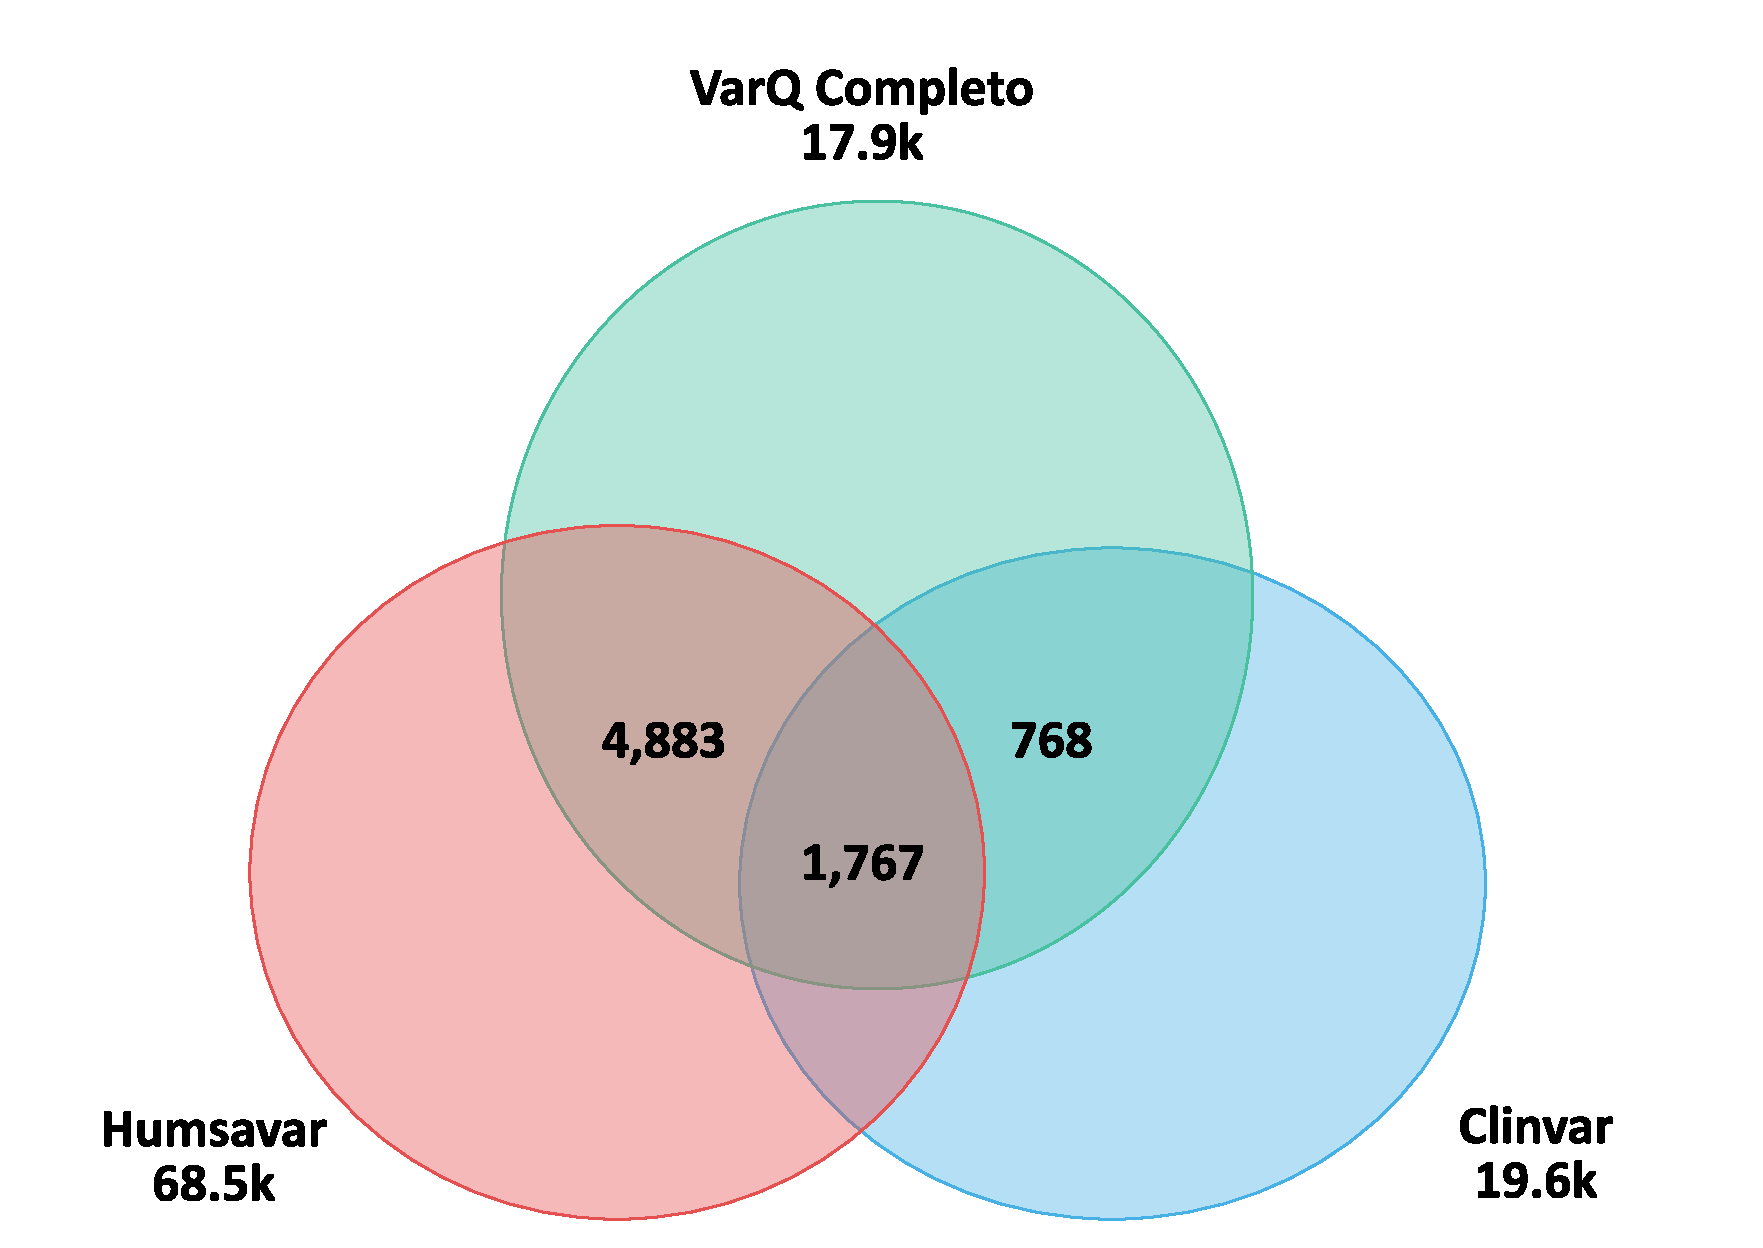
\includegraphics[scale=0.4]{documents/latex/figures/3/varq/interseccion_varq.pdf}
    \caption{Valores en la intersección del dataset VarQ con las tablas Clinvar y Humsavar.}
    \label{fig:interseccion_varq}
\end{figure}

Así, cruzamos los datos con las tablas filtradas Humsavar y Clinvar, y encontramos un subconjunto importante de variantes que no aparecían en ninguna de las dos fuentes. Estas variantes estaban rotuladas en su gran mayoría (94\%) como benignas, por lo que creemos que se consideraron como variantes benignas a todas aquellas a las que no se encontró un reporte. Decidimos remover estas variantes del dataset por considerar que si alguna de ellas estuviera rotulada incorrectamente introduciría ruido. Como puede observarse en la figura \ref{fig:interseccion_varq}, de las 17,869 variantes del dataset, logramos encontrar 2,535 en la tabla de Clinvar, de los cuales sólo 2,397 tenían un estado confirmado como patogénicas, y 138 como benignas. Cruzando el dataset con la tabla Humsavar encontramos una intersección de 6,650 variantes de los cuales 4,667 corresponden a patogénicas y 1,983 son benignas. Decidimos mantener la clasificación de Humsavar en la intersección de los tres conjuntos por considerarla de mayor confiabilidad dado que es un reporte único curado por expertos a diferencia de Clinvar que es una recopilación de variantes de diversa significación clínica, y a menudo presenta conflictos de anotación por discrepancias entre evidencias reportadas. Esto nos deja con un dataset Curado de 7,418 variantes de las cuales 5,377 son patogénicas y 2,041 son benignas. Denominaremos a este dataset \textit{VarQ Curado}. 


\subsection{Descripción estadística del dataset VarQ Curado}

A partir de VarQ Curado estudiaremos sus variables usando estadísticas descriptivas con el objetivo de evaluar la calidad del dataset. La idea es poder tener una noción de la dispersión de nuestros datos, sumado a la cobertura que tenemos de ellos sobre las variantes. En la tabla \ref{tab:descripcion_varq_cont} podemos ver distintas métricas sobre las variables continuas del dataset como la cantidad de variables con valor no nulo (count), la media de los valores (mean), el desvío estándar (std), el valor máximo (max) y los cuartiles. 

También sumamos a esta descripción el AUC univariado, es decir el área bajo la curva ROC tomando la variable ordenada como estimador de la respuesta.   

Un AUC cercano a 0.5 equivale a una variable de bajo poder predictivo, mientras que un AUC mayor a 0.5 corresponde a un predictor de la variable de respuesta (en este caso una variante patogénica), mientras que un AUC menor a 0.5 corresponde a un anti-predictor, es decir que invertir su respuesta equivale a un predictor de AUC mayor a 0.5.

\begin{table}[H]
\centering
\begin{tabular}{|l|l|l|l|l|l|l|l|l|}
\hline
Variable & avg  & std   & min    & 25\%  & 50\%  & 75\%  & max & AUC\\ \hline
SASA    & 32.11 & 39.15 & 0.0    & 0.67  & 15.21 & 52.15 & 246.41 & 0.34 \\ \hline
SASA\%  & 0.15  & 0.18  & 0.0    & 0.0   & 0.07  & 0.27  & 0.75 & 0.33  \\ \hline
BFACTOR & 56.45 & 71.76 & 0.0    & 19.77 & 37.34 & 61.14 & 755.61 & 0.46 \\ \hline
SWITCH  & 0.38  & 0.89  & 0.0    & 0.0   & 0.01  & 0.28  & 8.72 &  0.50  \\ \hline
AGG     & 5.02  & 17.61 & 0.0    & 0.0   & 0.0   & 0.16  & 100.0 &  0.51\\ \hline
CONS    & 0.33  & 0.19  & 0.13   & 0.25  & 0.3   & 0.37  & 4.77 & 0.43\\ \hline
ENE     & 2.91  & 4.84  & -12.64 & 0.26  & 1.51  & 3.89 & 57.21 & 0.68\\ \hline 
\end{tabular}
\caption{Descripción de variables continuas del dataset \textit{VarQ Curado}.}
\label{tab:descripcion_varq_cont}
\end{table}

Para el caso de las variables categóricas (PDB y 3DID), analizamos el valor con la frecuencia más alta (top). Para este tipo de variables quisimos también cuantificar su poder predictivo individual. El cálculo mediante AUC no es posible dado que los únicos valores posibles de estas variables son dos, por lo que no tiene sentido considerar modificar el \textit{threshold} en sólo un punto de corte. Por lo tanto decidimos calcular el \textit{Balanced Accuracy} como medida de poder predictivo considerando el valor de la variable como predictor de la variante. En la tabla \ref{tab:descripcion_varq_cat} podemos ver que el BACC de las variables 3DID y PDB es bajo. 

\pagebreak

El \textit{Balanced Accuracy} (BACC) es igual a:
\begin{equation*}
    \frac{1}{2} (\frac{TP}{P} + \frac{TN}{N})
\end{equation*}



\begin{table}[H]
\centering
\begin{tabular}{|l|l|l|l|}
\hline
Variable & top  & count & BACC \\ \hline
3DID    & False & 5939 & 0.51\\ \hline
PDB  & False  & 6696 & 0.49\\ \hline
\end{tabular}
\caption{Descripción de variables categóricas del dataset \textit{VarQ Curado}.}
\label{tab:descripcion_varq_cat}
\end{table}

Otro de los puntos importantes durante la exploración del dataset es la detección de variables con muy poca cobertura. En la figura \ref{fig:proporcion_nulos_varq} podemos observar como la variable de sitio activo (ACTIVE\_SITE) no posee datos para casi ninguna variante (aproximadamente el 95\%), mientras que la variable de conservación (CONS) no posee datos para el 63\% de las variantes. En base a estas observaciones decidimos remover la variable de sitio activo del dataset por considerarla muy poco relevante en términos de cobertura.

\begin{figure}[H]
    \centering
    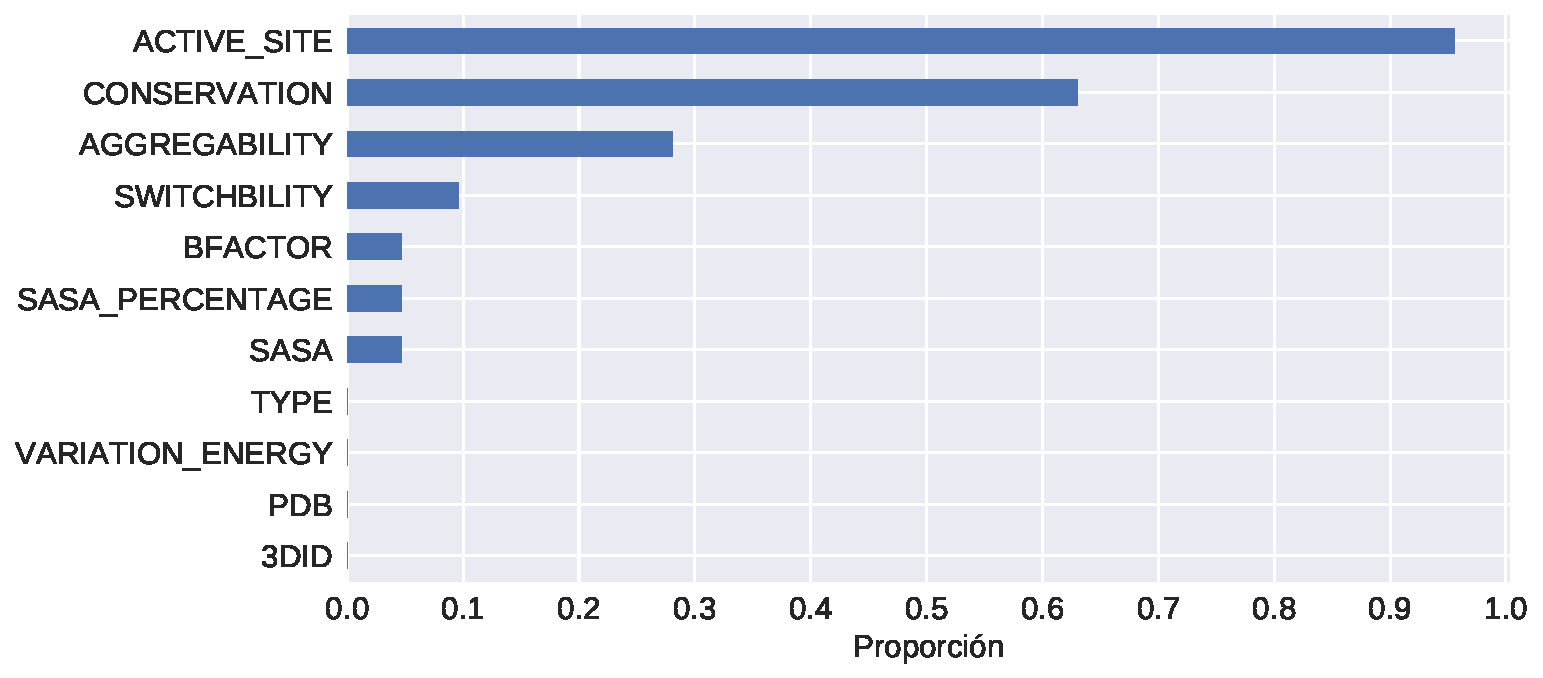
\includegraphics[scale=0.55]{documents/latex/figures/3/varq/proporcion_nulos.pdf}
    \caption{Proporción de variantes con valor nulo por variable del dataset VarQ Curado.}
    \label{fig:proporcion_nulos_varq}
\end{figure}

Otro factor importante a considerar es cuantas variables nulas tienen cada una de las variantes del dataset. En la figura \ref{fig:nulos_varq} podemos observar que existe aproximadamente un 5 \% de variantes que poseen 7 variables nulas de las 10 que contienen el dataset, es decir, prácticamente no tienen ningún tipo de información, y sólo el 2\% de las variantes posee el total de las variables cubiertas. Por el otro lado, casi el 90\% de las variantes tiene a lo sumo 3 variables nulas.

\begin{figure}[H]
    \centering
    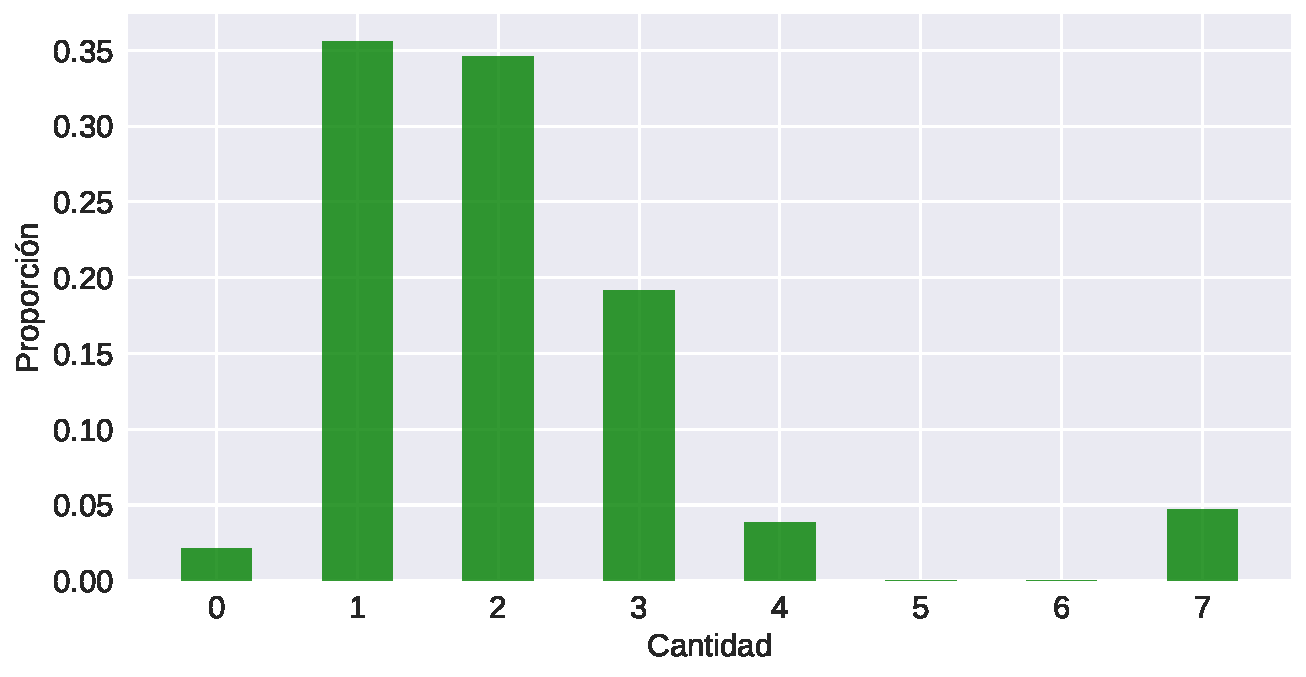
\includegraphics[scale=0.55]{documents/latex/figures/3/varq/nulos_varq.pdf}
    \caption{Histograma de cantidad de variables nulas del dataset VarQ Curado.}
    \label{fig:nulos_varq}
\end{figure}

Finalmente, también queremos conocer que tan correlacionadas se encuentras las variables. En la figura \ref{fig:varq_corrplot} vemos la correlación de Spearman que sirve para detectar relaciones monotónicas entre las variables, y así nos permite descartar variables muy similares que no aportan nueva información y ralentizan el entrenamiento del modelo. De esta forma encontramos que la variable SASA y SASA\_PERCENTAGE tienen una correlación de 0.98.

\begin{figure}[H]
    \centering
    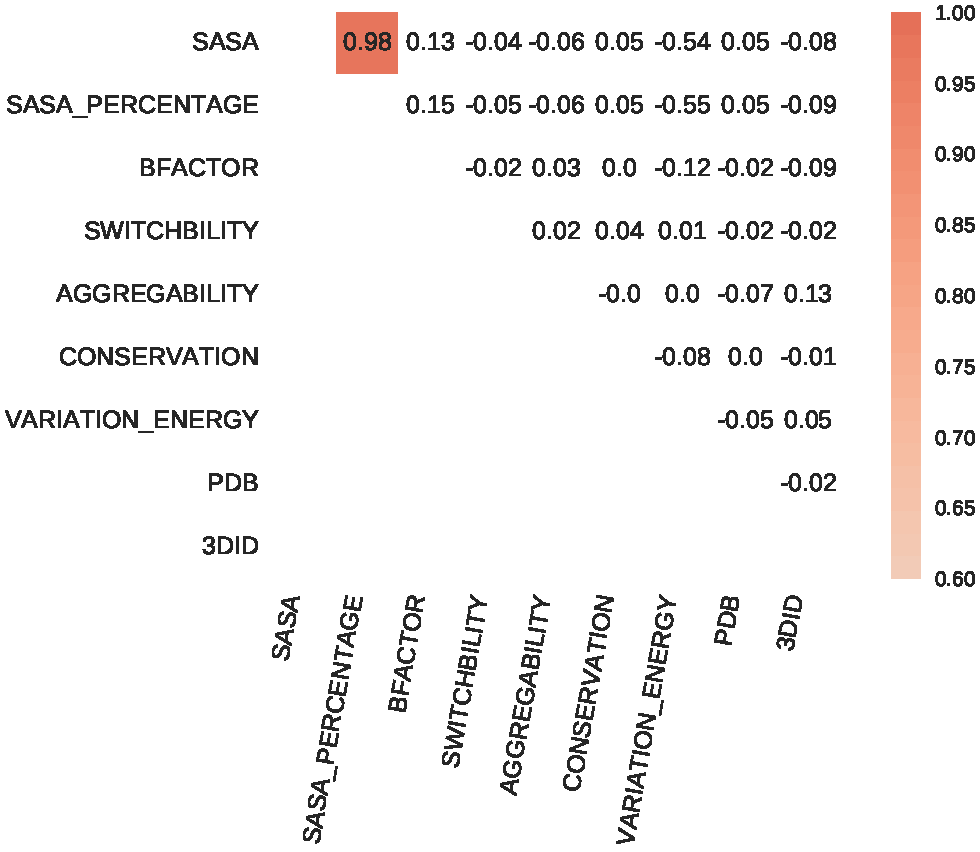
\includegraphics[scale=0.6]{documents/latex/figures/3/varq/varq_corrplot.pdf}
    \caption{Correlación de Spearman para las variables de VarQ Curado.}
    \label{fig:varq_corrplot}
\end{figure}

\pagebreak

\subsection{Modelo creado a partir del dataset Varq Curado}

Una vez definido el dataset, podemos emplear técnicas de aprendizaje automático con el objetivo de generar un predictor de variantes patogénicas. Cabe destacar, que en este dataset VarQ Curado hay una sobrerrepresentación de variantes patogénicas, es decir, que presenta un desbalance (mayor número de variantes patogénicas que benignas) que invierte las propociones observadas en el dataset VarQ Completo. De todas formas generaremos un modelo para poder evaluar de forma preliminar la dificultad del problema. 

Para esto recurrimos a diferentes algoritmos de aprendizaje automático: Support Vector Classifier (SVC), Regresión Logística y Random Forest. La construcción del pipeline para cada uno de estos algoritmos tuvo tres fases: 

\begin{itemize}
    \item \textbf{Creación del set de entrenamiento y de evaluación}: División (\textit{split}) estratificado (es decir, manteniendo las proporciones originales) del dataset, 66\% para entrenamiento y 33\% para evaluación. 
    \item \textbf{Imputación de las variables}: Se reemplazaron los valores nulos de cada variable por su mediana en caso de las continuas y por el valor más frecuente en el caso de las variables categóricas.
    \item \textbf{Estandarización}: Para el caso de los algoritmos paramétricos (Regresión Logística y SVM) se aplicó una estandarización robusta a outliers. Esta estandarización consiste en restar la mediana del valor y escalar los datos de acuerdo a la distancia intercuartil como se observa en la ecuación \ref{eq:robust_scaler}.
    
    \begin{equation}
        RobustScaling(x_i) = \frac{x_i - Q_2(\textbf{x})}{Q_3(\textbf{x}) - Q_1(\textbf{x})} 
        \label{eq:robust_scaler}
    \end{equation}
    
    
    
\end{itemize}

Luego del preprocesamiento, para cada uno de los algormitmos se realizó una búsqueda de hiperparámetros óptimos a partir de estos datos con la función \texttt{GridSearchCV} de la biblioteca \textit{Scikit-learn}. El objetivo de esta función es evaluar todas las combinaciones de hiperparámetros definidos en un diccionario y retornar el estimador que dio mejores resultados (de acuerdo a una métrica escogida, en este caso el área bajo la curva ROC). Esta métrica a su vez es evaluada a través de validación cruzada (\textit{3-fold Cross Validation}). 

Random Forest fue el mejor modelo con un AUC de 0.74. La Regresión Logística y SVC obtuvieron 0.71 y 0.70 respectivamente. La tabla \ref{tab:metrics_varq} muestra algunas métricas de interés obtenidos del modelo Random Forest para entender mejor los resultados del modelo basadas en el predictor generado. Las siguientes medidas son:

\begin{itemize}
    \item \textbf{Precisión}: La Precisión del modelo, está medida como la cantidad de positivos correctamente calificados (verdaderos positivos) sobre la cantidad de instancias calificadas como positivas (verdaderos positivos y falsos positivos).
    
    \begin{equation*}
        \frac{VP}{VP + FP}
    \end{equation*}
    
\pagebreak
    \item \textbf{Recall}: El Recall corresponde a la cantidad de verdaderos positivos sobre el total positivos (verdaderos positivos y falsos negativos.
    
    \begin{equation*}
        \frac{VP}{VP + FN}
    \end{equation*}
    
    \item \textbf{F1-Score}: El F1-Score es el promedio armónico entre la Precisión y el Recall. Usamos el promedio armónico de manera de afectar negativamente el resultado si alguno de los valores es especialmente bajo. Posee un rango de 0 a 1. 
    
    \begin{equation*}
        F_1 = \frac{2}{\tfrac{1}{\mathrm{recall}} + \tfrac{1}{\mathrm{precision}}} = 2 \cdot \frac{\mathrm{precision} \cdot \mathrm{recall}}{\mathrm{precision} + \mathrm{recall}}
    \end{equation*}
    
\end{itemize}

\begin{table}[H]
\centering
\begin{tabular}{|l|l|l|l|}
\hline
              & Precisión & Recall & F1-score \\ \hline
Benignas      & 0.57      & 0.26   & 0.36     \\ \hline
Patogénicas   & 0.77      & 0.93   & 0.84     \\ \hline
Promedio      & 0.71      & 0.74   & 0.71     \\ \hline
\end{tabular}
\caption{Reporte de métricas del modelo Random Forest usando el dataset VarQ Curado.}

\label{tab:metrics_varq}
\end{table}


En la figura \ref{fig:importance_varq} podemos observar la importancia de los features reportado por el algoritmo Random Forest, que ubica en primer lugar con una gran diferencia a la variable que hace referencia a la Variación de Energía, seguido por el BFACTOR y el porcentaje de SASA. Este dato también concuerda con sus valores de AUC univariado.

La precisión del modelo indica un número marcadamente bajo (0.57) en la clase benigna, lo que significa que casi una de cada dos variantes detectadas como benignas es en efecto patogénica. El Recall con respecto a las variantes benignas es de 0.26, es decir que el modelo sólo reconoce alrededor de un cuarto de las variantes benignas como tales. Por lo tanto podemos afirmar que este modelo tiene una tendencia a calificar las variantes como patogénicas, generando una gran cantidad de falsos positivos (o Error de tipo I). Es importante remarcar que estas métricas están generadas a partir de un una función de decisión o \textit{threshold} fijado por la versión del algoritmo usado. La curva ROC, o \textit{Receiver Operating Characteristic} nos permite esta evaluación, como podemos observar en la figura \ref{fig:auc_varq}.

\newpage

\begin{figure}[H]
\centering
\begin{subfigure}{0.8\textwidth}
    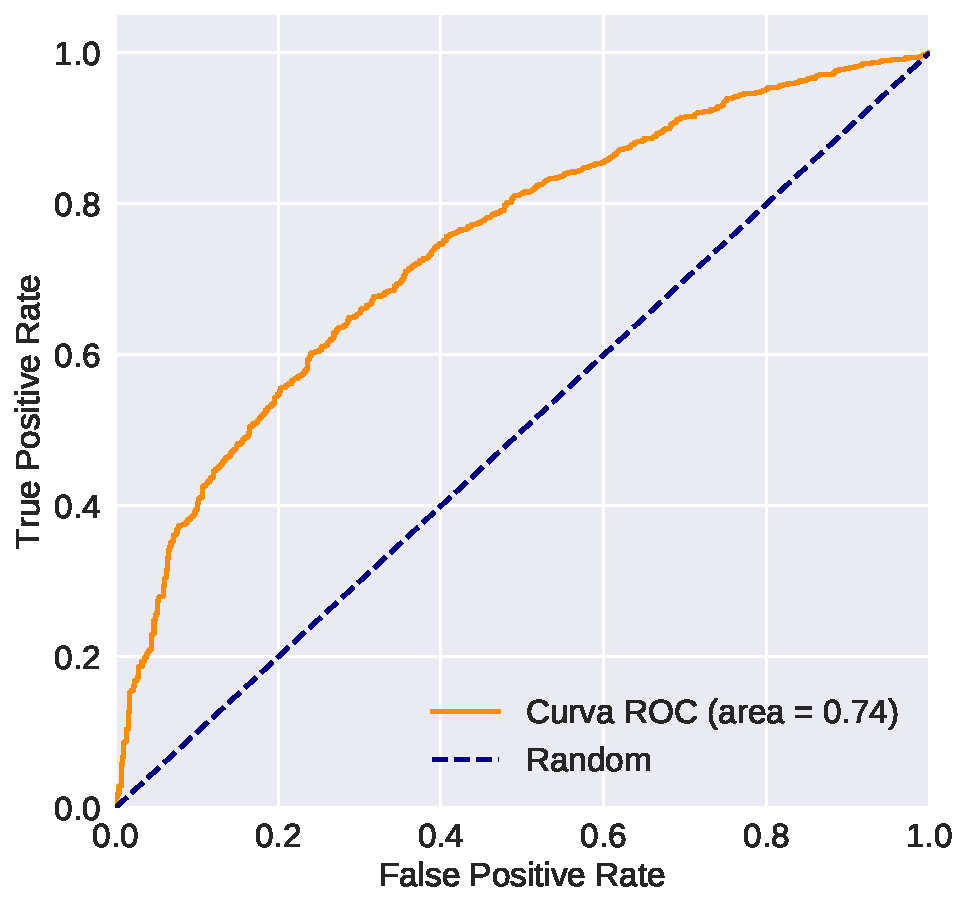
\includegraphics[width=\textwidth]{documents/latex/figures/3/varq/auc_varq.pdf}
    \caption{Curva ROC del algoritmo Random Forest del dataset VarQ. La línea punteada corresponde a la curva ROC de un estimador aleatorio, o \textit{Random}, cuyo AUC es igual a 0.5.}
    \label{fig:auc_varq}
\end{subfigure}
\begin{subfigure}{0.8\textwidth}
    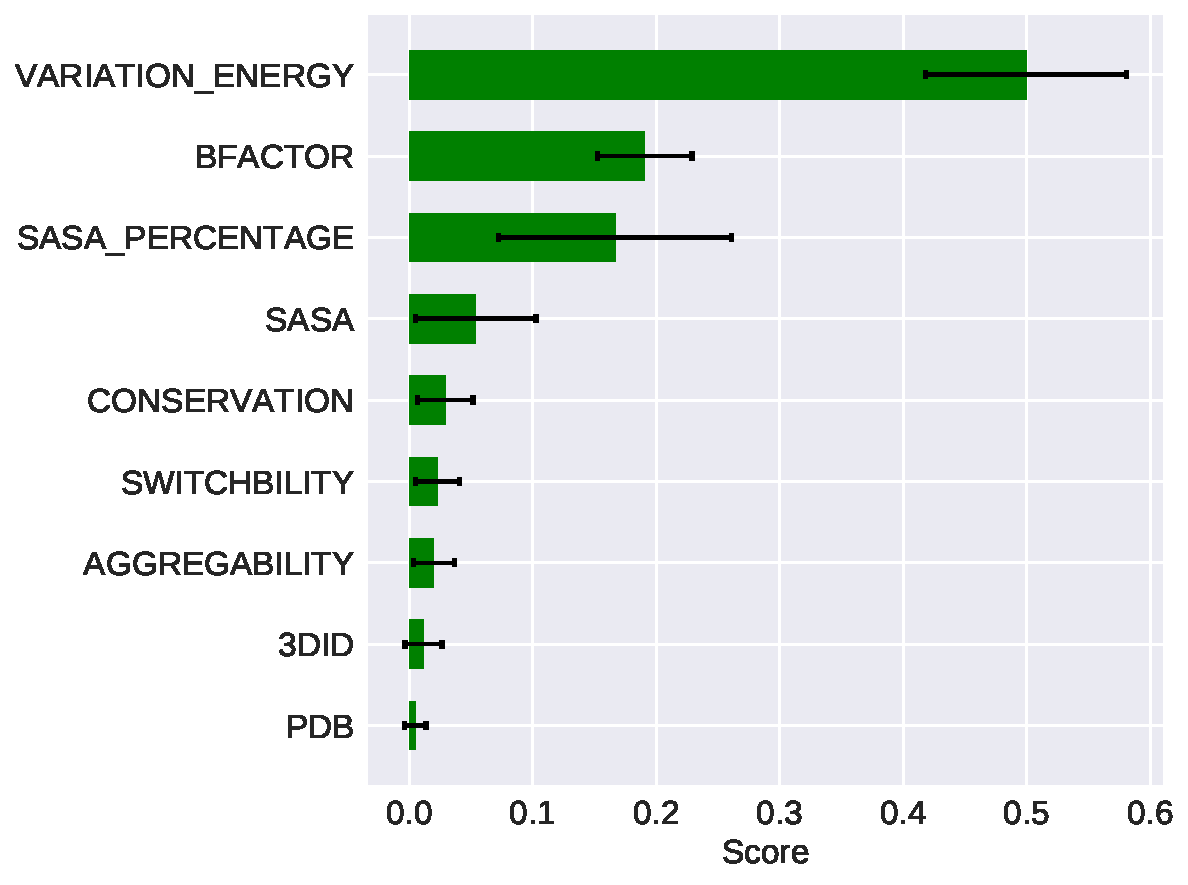
\includegraphics[width=\textwidth]{documents/latex/figures/3/varq/importances_varq.pdf}
    \caption{Los atributos del dataset VarQ en orden de importancia usando un modelo Random Forest. La barra de error corresponde al desvío estándar del \textit{Feature Importance} de cada uno de los árboles del modelo.}
    \label{fig:importance_varq}
\end{subfigure}
\end{figure}

\newpage

\section{Modelo usando Propiedades Estructurales de la Proteína}

En esta sección generamos un nuevo dataset buscando nuevas fuentes de información de carácter estructural de las proteínas. Estas variables provienen de dos fuentes principales:

\begin{itemize}
    \item El módulo ProtParam proveniente de la biblioteca Biopython
    \item La base de datos SNVBox del laboratorio Karchin
\end{itemize}

Para el análisis de estas variables usamos la tabla Humsavar. La tabla Humsavar (a Noviembre 2017) está compuesta originalmente por 75769 variantes (o ``mutantes'') de las cuales 39,653 son benignas (52\%), 28,855 (38\%) están asociadas a enfermedades y 7261 (10\%) no están clasificadas. 

\subsection{Extracción de variables usando Biopython}

La primera fuente que utilizamos, por su relativa practicidad de uso en la extracción de un conjunto de variables físico químicas de la proteína, fue el módulo ProtParam de la biblioteca Biopython. Esta biblioteca es un set de herramientas escritas en Python, desarrollada por colaboradores para el área de la bioinformática, y posee una licencia de uso libre \todo{[ref]}.
El nombre ProtParam proviene de \textit{Protein Parameters} (parámetros de la proteína) y está basado en la herramienta del server proteómico Expasy \todo{[ref]}. Requiere el \textit{accession number} de la proteína (identificador único) o una subsecuencia de la misma, para poder acceder a los parámetros calculados, que son los siguientes:

\begin{itemize}
    \item Punto isoeléctrico teórico (ISO\_POINT): pH en el que la proteína (o subsecuencia) tiene carga nula. 
    \item Aromaticidad (AROM): La frecuencia relativa de la subsecuencia Phe+Trp+Tyr (Fenilalanina, Triptófano y Tirosina). 
    \item Índice de inestabilidad (INST): Testea la estabilidad de la subsecuencia. Cualquier valor superior a 40 indica inestabilidad, es decir una corta semivida.  
    \item Flexibilidad (FLEX): Método de Flexibilidad implementado por Vihinen et Al.  
    \item Promedio de hidrofobicidad (GRAVY): La suma de valores de hidrofobicidad de cada uno de los aminoácidos que componen la subsecuencia de la proteína.
\end{itemize}

Para poder utilizar el módulo ProtParam recurrimos a Uniprot con el fin de conseguir el proteoma humano en formato FASTA. El formato FASTA fue desarrollado por David Lipman y William Pearson en 1985, y originalmente fue incluido en un programa del mismo nombre utilizado para el alineamiento múltiple de secuencias. Una archivo FASTA puede incluir diferentes secuencias, no necesariamente de aminoácidos, y cada una de estas secuencias posee una línea de descripción al comienzo que empieza con el símbolo $>$. Por ejemplo, así se ve la secuencia de la Ovoalbúmina, de la especie Gallus gallus (gallina), o en otras palabras, la principal proteína que encontramos en la clara de los huevos:

\begin{verbatim}
	>P01013 GENE X PROTEIN (OVALBUMIN-RELATED)
	QIKDLLVSSSTDLDTTLVLVNAIYFKGMWKTAFNAEDTREMPFHVTKQESKPVQMMCMNNSFNVATLPAE
	KMKILELPFASGDLSMLVLLPDEVSDLERIEKTINFEKLTEWTNPNTMEKRRVKVYLPQMKIEEKYNLTS
	VLMALGMTDLFIPSANLTGISSAESLKISQAVHGAFMELSEDGIEMAGSTGVIEDIKHSPESEQFRADHP
	FLFLIKHNPTNTIVYFGRYWSP
\end{verbatim}

\pagebreak

A partir del proteoma obtenido se extrajeron las secuencias correspondientes a las proteínas del dataset Humsavar, y para cada una de ellas se tomó una subsecuencia de la misma alrededor de la posición donde se produjo la variante.


    % \begin{figure}
    % \begin{textopo}
    %   \labelstyle{hl}{diamond}{Black}{Blue}{White}{}
    %   \sequence{PQALPSV[LQIAMAFGLAIGTLVQALG]HV%
    %   SGAH[([NNE,30]hl[box[Black,Blue]:Half loop[White]]=INPAVTVACL)]VGCHVSFLR}
    %   \Nterm{extra} \hideNterm \hideCterm \hidelegend \labelTM{1}{II}
    %   \labeloutside[right]{extra}
    % \end{textopo}
    % \caption{A `half loop' example}\label{fighalf}
    % \end{figure}


\vspace{2mm}
\todo{
TODO: Esquema de la subsecuencia
} 
\vspace{2mm}

Para cada una de los parámetros calculados en ProtParam, generamos dos variables que buscan reflejar la diferencia generada por la variante. 

\begin{itemize}
    \item Diferencia (DIFF) 
    $$|x - x_{var}|$$
    \item Cociente de logaritmos (LOG\_RATIO)
    $$\frac{\log{(x + 1)}}{\log{(x_{var} + 1)}}$$  
\end{itemize}

\subsection{Extracción de variables usando SNVBox}

Además de la información obtenida vía ProtParam, recurrimos a una base de datos llamada SNVBox \todo{[ref]}. Esta base de datos fue elaborada y es actualmente mantenida por el Karchin Lab de Universidad Johns Hopkins. Se encuentra en su versión 3.0 y sigue en desarrollo. \todo{Mencionar algunos papers que usaron esta base}. SNVBox posee alrededor de 90 variables consideradas relevantes para detectar el impacto biológico de un SNV \cite{Wong2011}, como datos sobre la estructura de la proteína, a nivel de aminoácido y también a nivel de los sitios de la proteína donde se encuentra la variante. Otra característica destacable de esta fuente es que posee dichas variables para todos los codones del exoma humano, lo que nos permitió una cobertura alta para las variantes del dataset con el que trabajamos. 

% Las variables utilizadas fueron:

% \subsubsection{Variables sobre cambios en la sustitución del Aminoácido (Estructura Primaria)}
% \begin{itemize}
%     \item Score BLOSUM (AABLOSUM)
%     \item Carga (AACharge)
%     \item Volumen (AAVolume)
%     \item Hidrofobia (AAHydrophobicity)
%     \item Score Grantham (AAGrantham)
%     \item Polaridad (Polarity)
%     \item Score Ex (AAEx)
%     \item Score PAM250 (AAPAM250)
%     \item Score MJ (AAMJ)
%     \item Score HGMD2003 (AAHGMD2003)
%     \item Score VB (AAVB)
%     \item Transición (Transition)
%     \item COSMIC
%     \item COSMICvsSWISSPROT
%     \item HAPMAP
%     \item COSMICvsHAPMAP
% \end{itemize}

% \subsubsection{Variables a nivel de Proteína (sin considerar sustitución)}

% \begin{itemize}
%     \item BINDING
%     \item ACTIVE\_SITE
%     \item SITE
%     \item LIPID
%     \item BINDING
%     \item ACT\_SITE
%     \item SITE
%     \item LIPID
%     \item METAL
%     \item CARBOHYD
%     \item DNA\_BIND
%     \item NP\_BIND
%     \item CA\_BIND
%     \item DISULFID
%     \item SE\_CYS
%     \item MOD\_RES
%     \item PROPEP
%     \item SIGNALP
%     \item TRANSMEM
%     \item COMPBIAS
%     \item REP
%     \item MOTIF
%     \item ZN\_FING
%     \item REGIONS
%     \item PPI
%     \item RNABD
%     \item TF
%     \item LOC
%     \item MMBRBD
% \end{itemize}

% \vspace{2mm}
% \todo{
% TODO:
% Diagrama de SNVBOX
% }
% \vspace{2mm}

\subsection{Generación del Dataset Estructural}

Luego del proceso del extracción de variables generamos un nuevo dataset cruzando estos atributos con las variantes de Humsavar. En el caso de los atributos relativos a los aminoácidos, pudimos cruzarlos usando la columna del dataset referente al identificador de la proteína, la posición de la variante, y el par de aminoácidos que se intercambiaron. Una vez agregados todas las variantes a la tabla Humsavar removimos todas aquellas variantes sin clasificación (etiqueta \textit{Unclassified}). El dataset resultante (denominado Dataset Estructural) está compuesto por 68,508 observaciones y 55 variables incluyendo la variable de respuesta (o tipo), de los cuales 39,653 son benignas (no se encontraron reportes de enfermedades en la literatura), y 28,855 variantes están asociadas a alguna enfermedad. 

\subsection{Descripción estadística del Dataset Estructural}

\subsubsection{Variables extraídas de Protparam}

\begin{table}[H]
\begin{tabular}{|l|l|l|l|l|l|l|l|}
\hline
Variable & mean & std & min & 25\% & 50\%  & 75\%  & AUC \\ \hline
AROM\_DIFF  & 0.02  & 0.02  & 0.00 & 0.00 & 0.00  & 0.01  & 0.41 \\ \hline
AROM\_LOG\_RATIO & 1.97 & 0.33 & 1.00 & 1.94 & 1.94  & 1.94  & 0.47 \\ \hline
ISO\_POINT\_DIFF & 0.69  & 0.98 & 0.00  & 0.00 & 0.17  & 1.22  & 0.44 \\ \hline
ISO\_POINT\_LOG\_RATIO & 2.00 & 0.08 & 1.69 & 1.99 & 2.00  & 2.01  & 0.49 \\ \hline
GRAVY\_DIFF & 0.23 & 0.17 & 0.00 & 0.09 & 0.20  & 0.33  & 0.45 \\ \hline
GRAVY\_LOG\_RATIO & 1.99x10$^{12}$ & 1.24x$10^{14}$ & -3.39x10$^{15}$ & 1.43 & 1.94 & 2.43 & 0.52 \\\hline
INST\_DIFF & 14.02 & 13.27 & 0.00 & 4.20 & 10.09 & 20.10 & 0.51 \\ \hline
INST\_LOG\_RATIO & 2.06 & 2.27 & -84.77 & 1.96 & 2.01  & 2.09  & 0.52 \\ \hline
FLEX\_DIFF & 0.01 & 0.01 & 0.00 & 0.00 & 0.01  & 0.01  & 0.46 \\ \hline
FLEX\_LOG\_RATIO & 2.00 & 0.01 & 1.97 & 1.99 & 2.00  & 2.01  & 0.53 \\ \hline
\end{tabular}
\end{table}

% \newpage

\subsubsection{Variables extraídas de SNVBox relativas a sustitución de aminoácidos}

\begin{table}[H]
\begin{tabular}{|l|l|l|l|l|l|l|l|}
\hline
Variable & mean   & std    & min    & 25\%  & 50\%   & 75\%   & AUC    \\ \hline
CHARGE            & 0.00  & 0.71   & -2.00  & 0.00  & 0.00   & 0.00   & 0.50   \\ \hline
VOLUME            & -0.16  & 1.70   & -5.59  & -1.40 & -0.16  & 0.96   & 0.52   \\ \hline
HYDROPHOBICITY    & -0.63  & 6.81   & -15.70 & -3.10 & -0.40  & 1.90   & 0.48  \\ \hline
GRANTHAM          & 79.96  & 48.06  & 5.00   & 43.00 & 74.00  & 102.00 & 0.37 \\ \hline
POLARITY          & -0.25  & 2.72   & -8.10  & -2.20 & -0.10  & 1.10   & 0.48   \\ \hline
EX                & 28.99  & 10.95  & -1.00  & 21.00 & 29.00  & 35.00  & 0.65  \\ \hline
PAM250            & 0.16   & 1.68   & -5.40  & -1.00 & 0.20   & 1.40   & 0.64   \\ \hline
BLOSUM            & -0.58  & 1.65   & -4.00  & -2.00 & -1.00  & 1.00   & 0.65   \\ \hline
JM                & 0.80   & 1.24   & -1.73  & -0.50 & 1.05   & 1.66   & 0.60   \\ \hline
VB                & 19.78  & 14.64  & 0.00   & 8.00  & 17.00  & 29.00  & 0.58  \\ \hline
TRANSITION        & 0.00   & 0.00   & 0.00   & 0.00  & 0.00   & 0.00   & 0.53   \\ \hline
\end{tabular}
\end{table}

\subsubsection{Variables extraídas de SNVBox relativas a proteínas}

Estas variables son todas categóricas de tipo \textit{Boolean} por lo que destacamos dos datos de relevancia. Todas estas variables tienen un coverage del 31.5\% del dataset, y cada una de ellas poseen valor Falso para un porcentaje superior al 90\% de las variantes de la tabla, exceptuando la variable \textbf{TRANSMEM} (82\%), \textbf{REP} (87\%), \textbf{REGIONS} (70\%) y \textbf{PPI} (87\%).


\subsubsection{Correlación entre las variables}

\begin{figure}[H]
    \centering
    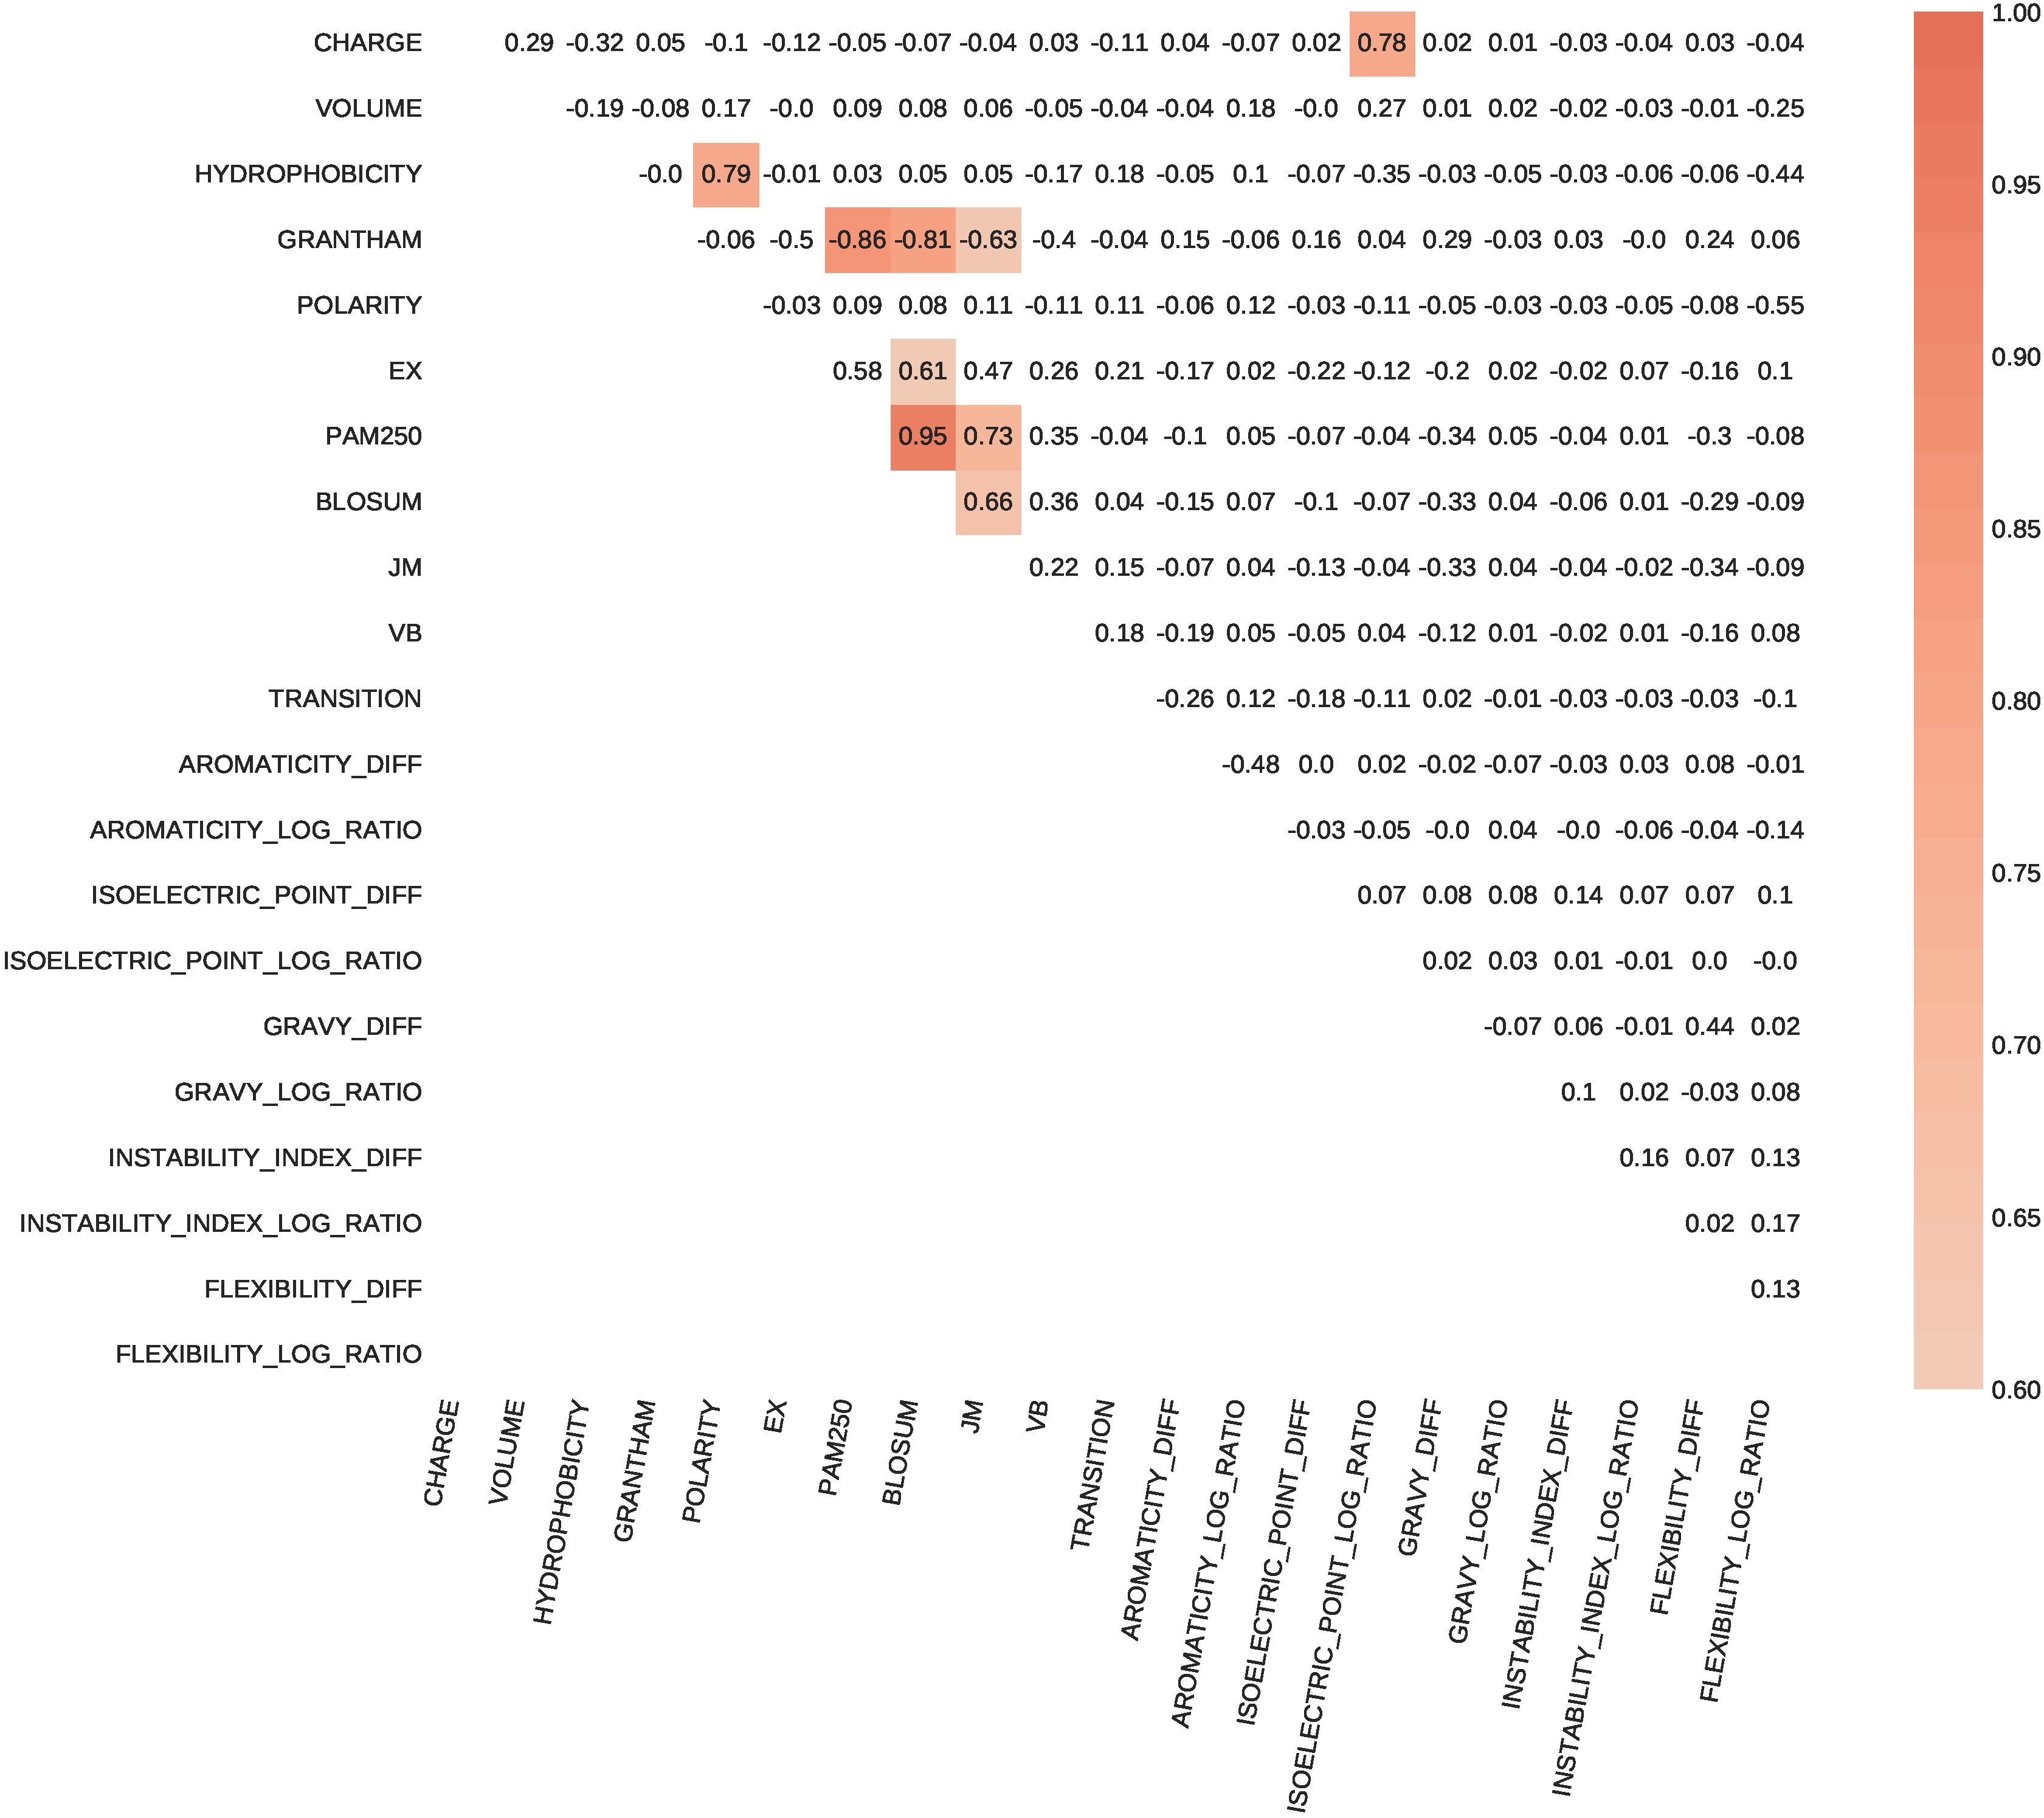
\includegraphics[scale=0.25]{documents/latex/figures/3/structural/structural_corr.pdf}
    \caption{Correlación de Spearman para las variables del Dataset Estructural.}
    \label{fig:corrplot_structural}
\end{figure}

Por último, deseamos analizar la correlación entre las variables. Para esto usamos la correlación de Spearman dado que nos permite identificar correlaciones monotónicas. En la figura \ref{fig:corrplot_structural} podemos apreciar un cluster principal de variables altamente correlacionadas: Las matrices de sustitución (Grantham, BLOSUM, JM, y EX). Por otro lado, encontramos a las variables POLARITY y HYDROPHOBICITY correlacionadas entre sí (0.79), como también a las variables CHARGE y ISOELECTRIC\_POINT\_LOG\_RATIO (0.78).


% \subsubsection{Análisis de reducción de dimensionalidad}

% Una de las formas que nos permite ver que tan bien las variables de este dataset están separando nuestros tipos de SNPs, es usar reducción de dimensionalidad. El primer método que probamos fue el análisis de componentes principales (PCA), con el que generamos dos componentes, que son combinaciones lineales de nuestras variables iniciales de forma de maximizar la varianza, es decir el par de componentes que mejor explican la información completa.


% \newpage


\subsection{Generación del Modelo}

Con este dataset generamos un modelo basado en un predictor Random Forest. 
Se eligió inicialmente este tipo de predictor por ser el que obtuvo los mejores resultados en el dataset VarQ Curado con respecto a otros predictores (SVMs y Regresión Logística). Otras de las ventajas que aporta este modelo es su facilidad para explicar la importancia de las variables y su relativa baja complejidad computacional \todo{[Citar?]}. 

Para esto volvimos a generar un Pipeline muy similar al de la sección anterior:

\begin{itemize}
 
\item \textbf{Imputación}: Las variables se imputaron usando la mediana en el caso de las variables continuas, y con el valor más frecuente para las variables categóricas. 
\item \textbf{Escalado}: Las variables no fueron escaladas al no ser necesario en algoritmos de clasificacion basados en árboles de decisión, dado que se evalúan las variables de forma independiente. 
\item \textbf{Búsqueda de Hiperparámetros}: Para la búsqueda de hiperparámetros usamos \textit{Grid-Search} (búsqueda ``en cuadrícula'').
\end{itemize}


\subsection{Resultados del Modelo Estructural}

Como puede observarse en la figura \ref{fig:auc_structural}, a partir de este modelo se obtuvo un AUC de 0,71, que supera lo obtenido por el modelo usando el dataset VarQ. Las métricas observadas en la tabla \ref{structural_table} permiten dar cuenta de una precisión del 65\% con respecto a las observaciones patogénicas, es decir, el modelo está reportando una 36\% cantidad de variantes como patogénicas que no lo son (también conocido como error de tipo I), y un recall de 47\%, lo que indica que existe un 53\% de variantes patogénicas en nuestro dataset que no están siendo detectadas por nuestro modelo (error de tipo II). 

\begin{table}[H]
\centering
\begin{tabular}{|l|l|l|l|}
\hline
              & Precisión & Recall & F1-score \\ \hline
Benignas      & 0.68      & 0.81   & 0.74     \\ \hline
Patogénicas   & 0.65      & 0.47   & 0.54     \\ \hline
Promedio      & 0.66      & 0.67   & 0.66     \\ \hline
\end{tabular}
\caption{Métricas del modelo Random Forest aplicado al dataset estructural.}
\label{structural_table}
\end{table}


\subsection{Importancia de los atributos}

El algoritmo Random Forest nos permite identificar los mejores atributos dado su rango en cada uno de los árboles del clasificador. En este caso, podemos ver que los primeros cuatro atributos refieren a matrices de sustitución. Los siguientes features pertenecen a ProtParam, como la aromaticidad, la polaridad y la hidrofobicidad. La hidrofobicidad, o la capacidad de repeler el agua de la subsecuencia de los aminoácidos, es uno de las variables consideradas relevantes para definir la patogenicidad de una proteína, de acuerdo al paper de Wang et al. \cite{Wang2016}. También en la figura \ref{fig:importances_structural}, se observan variables con un nivel de importancia muy similar, como es el caso de PAM250, EX, BLOSUM y GRANTHAM. Estas variables corresponden a matrices de sustitución. y en la figura \ref{fig:corrplot_structural} podemos corroborar que existe una alta correlación entre ellas.

\pagebreak

\begin{figure}[H]
\centering
\begin{subfigure}[b]{0.8\textwidth}
    \centering
    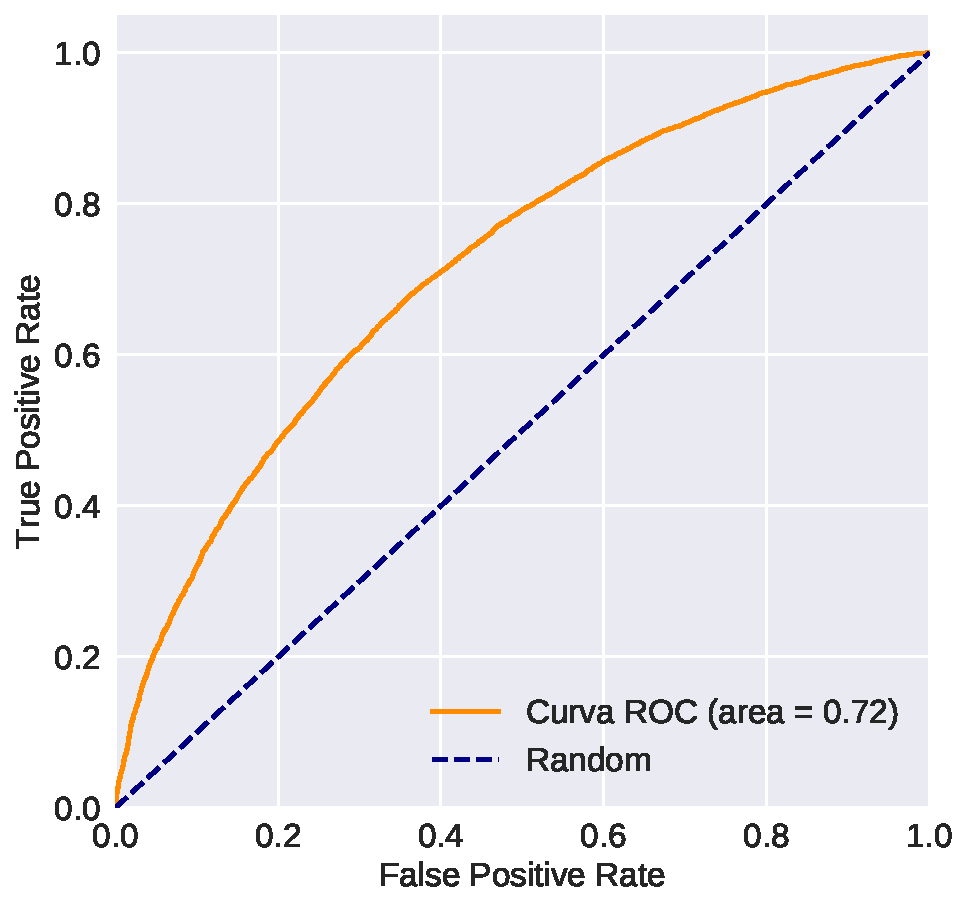
\includegraphics[width=\textwidth]{documents/latex/figures/3/structural/auc_structural.pdf}
    \caption{Curva AUC del algoritmo Random Forest aplicado al dataset estructural. La línea punteada corresponde a un predictor Random.}
    \label{fig:auc_structural}
\end{subfigure}

\hfill
\hfill

\begin{subfigure}[b]{\textwidth}
    \centering
    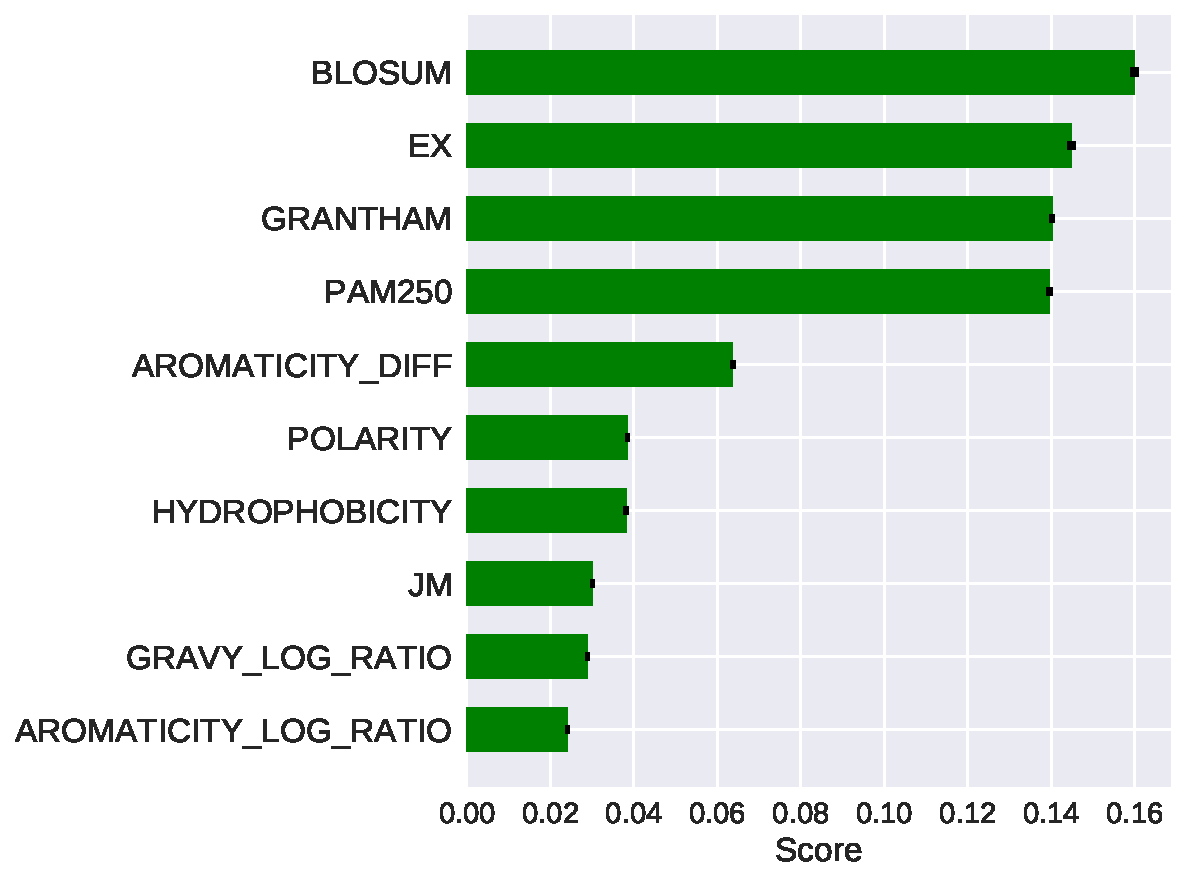
\includegraphics[width=\textwidth]{documents/latex/figures/3/structural/importances_structural.pdf}
    \caption{Los 10 atributos más importantes del modelo Random Forest usando el dataset estructural.}
    \label{fig:importances_structural}
\end{subfigure}

\end{figure}

\section{Modelo usando Variables Genómicas}

Otra de las preguntas que nos hicimos fue si las variables genómicas podían hacer un aporte al modelo, siendo en los genes es donde se produce la mutación que finalmente da origen a la variante en la proteína. En la tabla Humsavar existe, para la mayoría de las mutaciones, el identificador rsID o Reference SNP ID. Un identificador rsID agrupa los distintos reportes que hacen referencia a la misma posición dentro del mismo genoma de referencia (hg19/GRCh37). A partir de este identificador fue posible obtener de la base de datos dbSNP (Versión snp150) datos como el cromosoma, la posición y el cambio de nucleótido de la variante. 

\subsection{Variables de Conservación}

En la literatura encontramos que dos de las variables genómicas asociadas a la conservación eran las que daban mejores resultados (modelos FATHMM-MKL \cite{Shihab2015} o VEST \cite{Carter2013}). Esta \textit{conservación} es un término biológico que refiere a las secuencias conservadas, es decir secuencias tanto genéticas como proteicas que se mantienen de forma similar o idéntica en muchas especies que poseen un ancestro evolutivo en común (esta \textit{familia} de especies también se denomina árbol filogenético). En particular, la composición de estas variables consiste en alineamientos múltiples de secuencias genéticas (MSA) de 46 especies de vertebrados, incluyendo Homo Sapiens y otras como Felis catus (gato doméstico), Danio renus (pez cebra) y Equus Caballus (el caballo). En base a este alineamiento se usan dos medidas distintas de conservación:
\begin{itemize}
    \item \textbf{PhastCons-46-Way} \cite{siepel2005evolutionarily}
    \item \textbf{PhyloP-46-Way} \cite{Pollard2010}
\end{itemize}
Ambas variables buscan detectar aquellas regiones en el genoma con mayor nivel de conservación entre las distintas especies. Decidimos incluir en nuestro dataset ambas medidas de conservación, usando el Table Browser de la Universidad de California, Santa Cruz \cite{Karolchik2004}.

\subsection{Variables relativas a la Clase Funcional}

También tomamos en consideración la función de la posición dentro del gen. La base de datos dbSNP define cada SNP de acuerdo a su clase funcional. Si la variación se encuentra cerca del intervalo de un transcripto, pero no en la región codificante, la clase funcional va a depender de la posición de la variación relativa a la estructura del transcripto \cite{Ostell2007}.  Por otro lado, si la variación se encuentra en una zona codificante, la clase funcional se va a definir en base a si el alelo de la variación va a resultar en una sustitución sinónima (es decir, el nuevo codón va a formar el mismo aminoácido), una sustitución no sinónima (es decir, el nuevo codón va a formar un aminoácido distinto) o una sustitución sin sentido (en donde la mutación genera un codón de terminación prematuro). En base a esta información generamos variables \textit{dummies}, que indican con 1 o 0 la existencia de un lugar con una determinada clase funcional.


% , que puede ser:
 
% \begin{itemize}
%     \setlength\itemsep{0em}
%     \item INTRON
%     \item MISSENSE
%     \item NEAR-GENE
%     \item NCRNA
%     \item CODING-SYNON
%     \item UNTRANSLATED
%     \item NONSENSE
%     \item SPLICE
%     \item STOP-LOSS
% \end{itemize}

\subsection{Extracción de variables usando SNVBox}

Por último, usamos variables genómicas del dataset SNVBox, en particular de la tabla \texttt{Exon\_Features}. Las variables usadas son:
\begin{itemize}
    \item ExonConservation (CONS): Score de Conservación para el exón completo calculado a partir de una alineación filogenética a 46 vías.
    \item ExonHapMapSnpDensity (HAPMAP\_SNP\_DEN): Número de SNPs (verificados en HapMap) en el exón donde ocurre la mutación dividido por la longitud del exón.
    \item ExonSnpDensity (SNP\_DEN): Número de SNPs en el exón donde ocurre la mutación dividido por la longitud del exón.
\end{itemize}

Estas variables estaban definidas a nivel de exón, por lo que cada una de ellas poseía dos  identificadores UID (identificador de la secuencia proteica) y EXON (identificador del exón dentro de cada transcripto mRNA). Estos identicadores permitían en cruce con la tabla \texttt{Transcript\_Exon} dentro de la base SNVBox. Esta tabla a su vez obtener el número del cromosoma del exón, y la posición de inicio y fin del exón dentro del cromosoma. Una vez obtenidos estos datos, pudimos extraer todos los rsID dentro de esa subsecuencia. Finalmente, le asignamos el valor de la variable a todos los rsIDs en nuestra tabla Humsavar. Para algunos casos obtuvimos más de un valor para un mismo rsID, por lo que tomamos la decisión de promediarlos.

\todo{Esquema de acceso a la variable}

\subsection{Construcción del Dataset Genómico}

Con los atributos mencionados anteriormente, pudimos cruzar la información usando la columna rsID (Reference SNP cluster ID). Esta columna identifica a un cluster de variaciones de un sólo nucleótido que pertenece a la misma posición en el genoma (o conjunto de posiciones) \cite{Ostell2007}. Filtramos las variantes de Humsavar que no poseían este identificador. Finalmente el Dataset Genómico se compone de 55,382 variantes de las cuales 37,572 (68\%) variantes son benignas y 17,807 (32\%) son patogénicas.

\subsection{Descripción estadística del Dataset Genómico}

\subsubsection{Variables de Conservación}
\begin{table}[H]
\centering
\begin{tabular}{|l|l|l|l|l|l|l|l|l|}
\hline
Variable & count & mean   & std    & min    & 25\%  & 50\%   & 75\%   & max    \\ \hline
PHYLOP46WAY &  54389 &  2.16 &  2.29 & -8.22 &  0.29 &  1.81 &  4.23 &  6.42 \\ \hline
PHASTCONS46WAY &  54389 &  0.67 &  0.44 &  0.00 &  0.06 &  0.99 &  1.00 &  1.00 \\ \hline
\end{tabular}
\end{table}



\subsubsection{Variables relativas a la Clase Funcional}
\begin{table}[H]
\begin{tabular}{|l|l|l|l|l|l|l|l|l|}
\hline
Variable     & count    & mean & std  & min  & 25\% & 50\% & 75\% & max  \\ \hline
INTRON       & 54849.00 & 0.14 & 0.34 & 0.00 & 0.00 & 0.00 & 0.00 & 1.00 \\ \hline
MISSENSE     & 54849.00 & 0.99 & 0.10 & 0.00 & 1.00 & 1.00 & 1.00 & 1.00 \\ \hline
NEAR-GENE    & 54849.00 & 0.06 & 0.24 & 0.00 & 0.00 & 0.00 & 0.00 & 1.00 \\ \hline
NCRNA        & 54849.00 & 0.17 & 0.38 & 0.00 & 0.00 & 0.00 & 0.00 & 1.00 \\ \hline
CODING-SYNON & 54849.00 & 0.02 & 0.14 & 0.00 & 0.00 & 0.00 & 0.00 & 1.00 \\ \hline
UNTRANSLATED & 54849.00 & 0.05 & 0.23 & 0.00 & 0.00 & 0.00 & 0.00 & 1.00 \\ \hline
NONSENSE     & 54849.00 & 0.01 & 0.07 & 0.00 & 0.00 & 0.00 & 0.00 & 1.00 \\ \hline
SPLICE       & 54849.00 & 0.00 & 0.02 & 0.00 & 0.00 & 0.00 & 0.00 & 1.00 \\ \hline
STOP-LOSS    & 54849.00 & 0.00 & 0.01 & 0.00 & 0.00 & 0.00 & 0.00 & 1.00 \\ \hline
\end{tabular}
\end{table}

\subsubsection{Variables extraídas de SNVBox a nivel de Exón}
\begin{table}[H]
\begin{tabular}{|l|l|l|l|l|l|l|l|l|}
\hline
Variable         & count    & mean & std  & min  & 25\% & 50\% & 75\% & max  \\ \hline
CONS             & 54326.00 & 0.65 & 0.09 & 0.14 & 0.59 & 0.66 & 0.72 & 0.90 \\ \hline
SNP\_DEN         & 54326.00 & 0.06 & 0.10 & 0.00 & 0.03 & 0.04 & 0.06 & 1.04 \\ \hline
HAPMAP\_SNP\_DEN & 54326.00 & 0.00 & 0.00 & 0.00 & 0.00 & 0.00 & 0.00 & 0.04 \\ \hline
\end{tabular}
\end{table}





\subsubsection{Correlación entre las variables}

\begin{figure}[H]
    \centering
    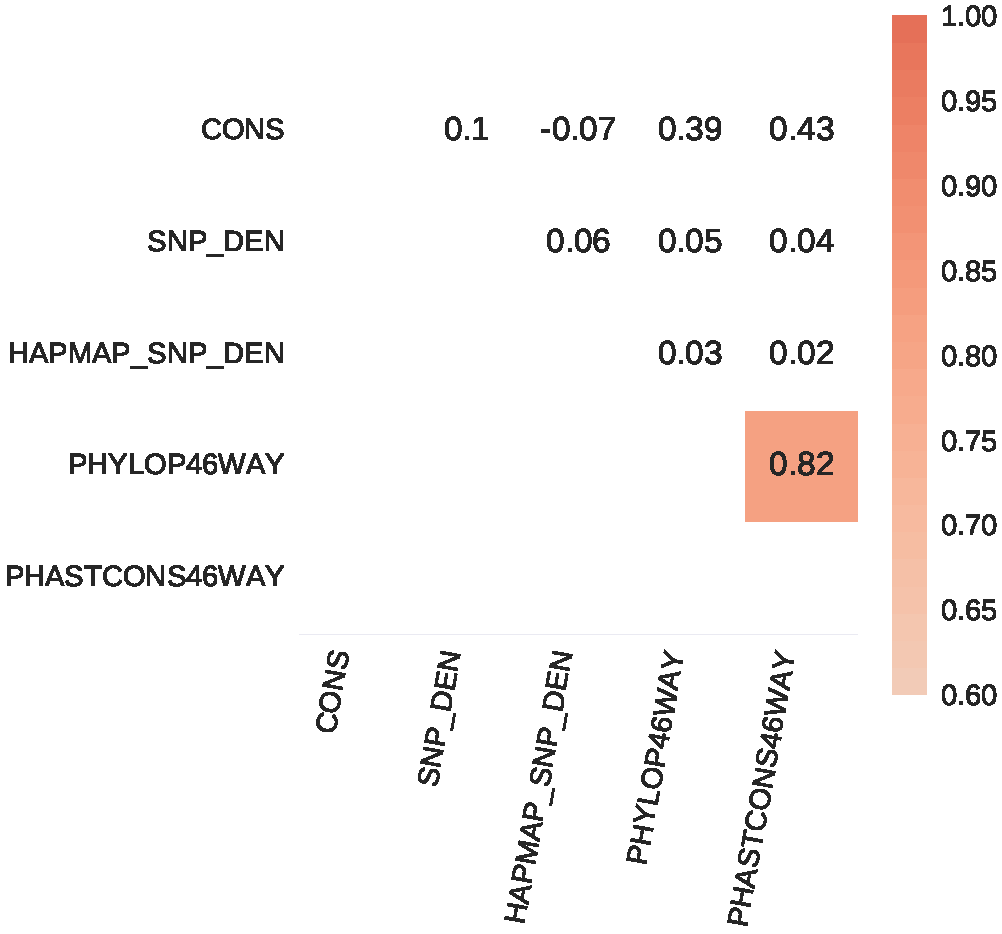
\includegraphics[scale=0.6]{documents/latex/figures/3/genomic/genomic_corr.pdf}
    \caption{Correlación de Spearman para las variables continuas del Dataset Genómico.}
    \label{fig:corrplot_genomic}
\end{figure}

\subsection{Generación del Modelo}

Luego de realizada la exploración del dataset generamos un modelo basado en Random Forest. Volvimos a utilizar este algoritmo debido a los resultados obtenidos en el dataset VarQ y para facilitar la comparación entre datasets. Este modelo se compone de un \textit{pipeline} de dos fases principales: Imputación, y Entrenamiento. En la fase de imputación se reemplazo los valores nulos por el valor más frecuente en el caso de las variables categóricas (por ejemplo las referentes a las clases funcionales) y con la mediana para las variables continuas. Las variables no fueron escaladas dado que en los algoritmos que involucran árboles de decisión, como Random Forest, las variables son evaluadas una a una y por lo tanto la escala de cada una de ellas no afecta la evaluación de las demás.

Como se puede observar en la figura \ref{fig:auc_genomic} obtuvimos un AUC de 0,89. Este resultado es muy superior a los obtenidos en los modelos anteriores, tanto en VarQ Curado como el Dataset Estructural. 
Analizando la importancia de las variables en el modelo, en la figura \ref{fig:importances_genomic} podemos observar que las variables de conservación están en los primeros dos puestos, confirmando lo obtenido por los trabajos de investigación antes mencionados. Por otro lado, esto genera un interrogante adicional: ¿Cuál es la razón por la que la variable \textit{Conservación} del dataset VarQ no genera un rendimiento similar?

Como podemos observar en la figura \ref{fig:importances_genomic}, el poder informativo de las variables de conservación es muy similar. La pregunta que nos hacemos en este caso es: ¿Las dos primeras variables de conservación están en los primeros dos lugares porque están altamente correlacionadas o aportan diferente información sobre las variables? En la figura \ref{fig:corrplot_genomic} podemos observar que estas variables se encuentran correlacionadas. 

\newpage

\begin{figure}[H]
\centering
\begin{subfigure}[b]{0.8\textwidth}
    \centering
    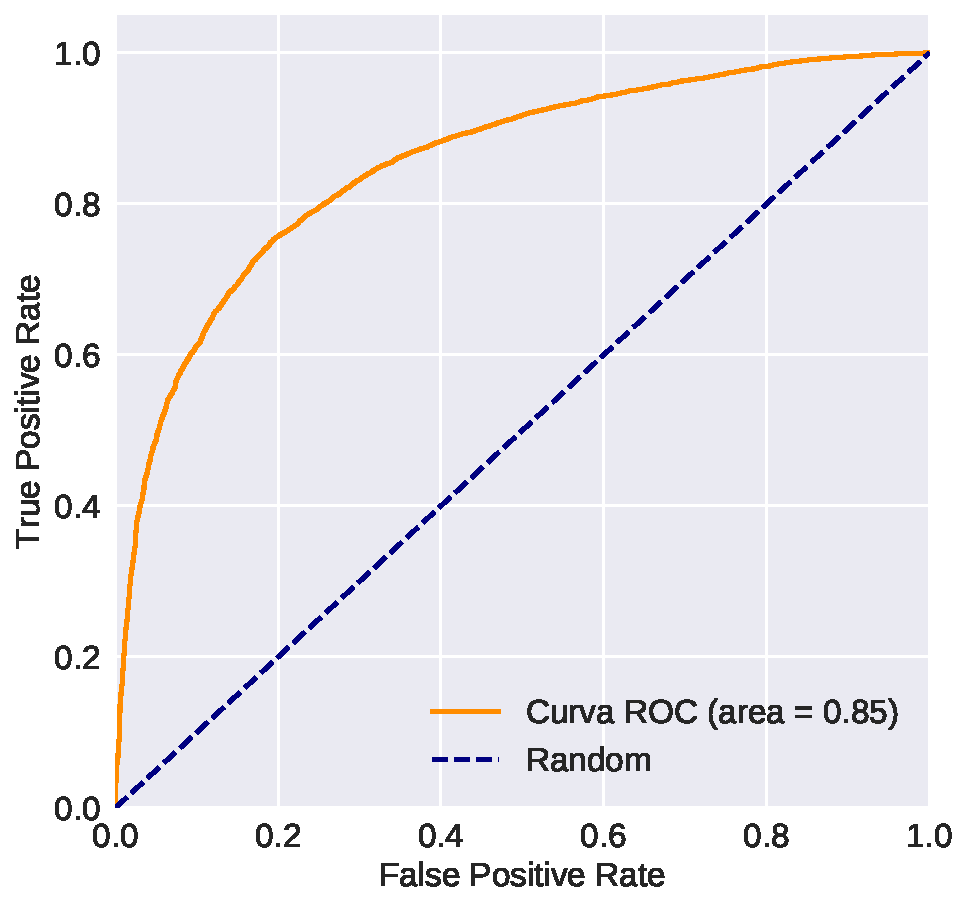
\includegraphics[width=\textwidth]{documents/latex/figures/3/genomic/auc_genomic.pdf}
    \caption{Curva AUC del algoritmo Random Forest aplicado al dataset genómico. La línea punteada corresponde a un predictor Random.}
    \label{fig:auc_genomic}
\end{subfigure}

\hfill
\hfill

\begin{subfigure}[b]{\textwidth}
    \centering
    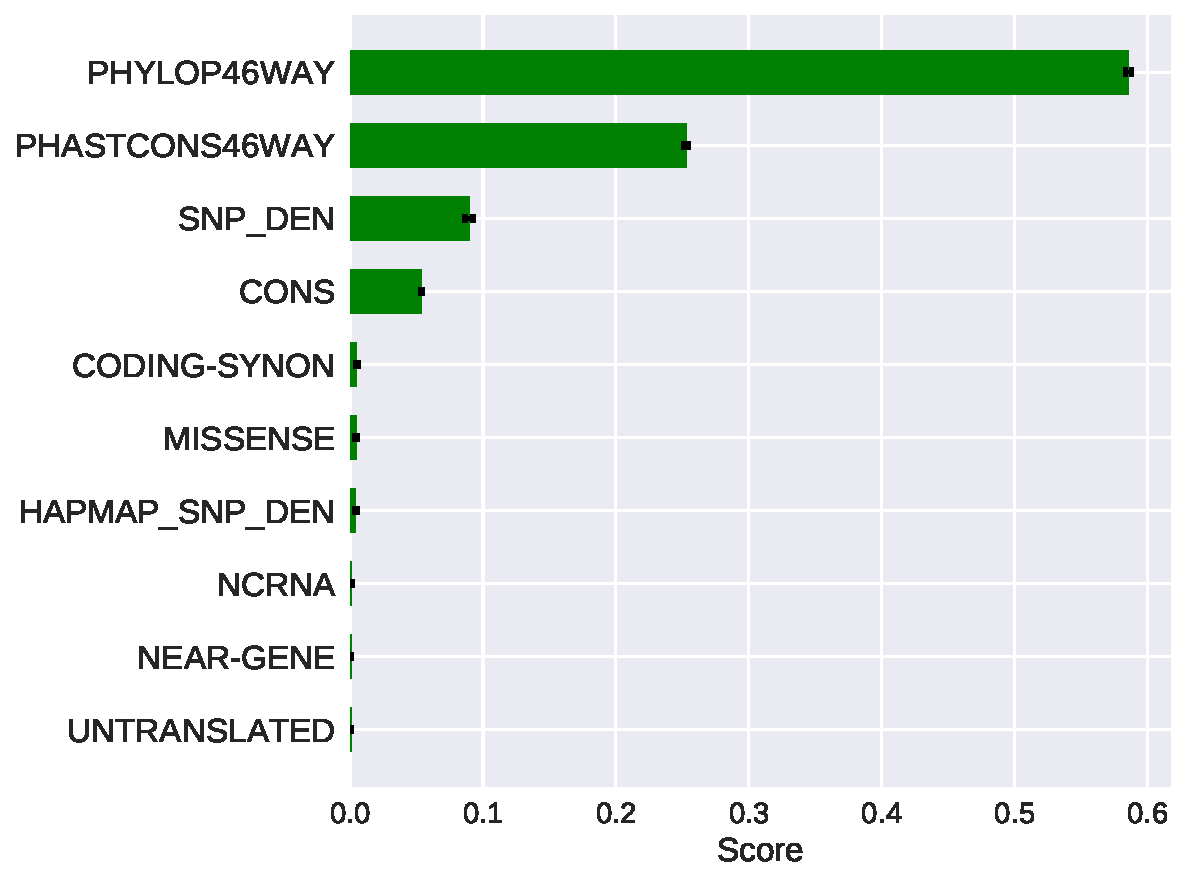
\includegraphics[width=\textwidth]{documents/latex/figures/3/genomic/importances_genomic.pdf}
    \caption{Los 10 atributos más importantes del modelo Random Forest usando el dataset genómico.}
    \label{fig:importances_genomic}
\end{subfigure}

\end{figure}


% \subsection{Descripción}
% \subsection{Correlación}
% \subsection{Resultados}


% \newpage

\section{Integrando el dataset estructural y el genómico}

Finalmente, unimos los dos conjuntos de variables para ver si la integración de ambos datasets representan una mejora frente a los resultados del modelo genómico. A este nuevo dataset lo denominamos Dataset Integral. Las variantes usadas fueron las encontradas en la tabla Humsavar. 

\subsection{Generación del Modelo}

Para este modelo preliminar volvimos a utilizar Random Forest, repitiendo las dos fases de imputación y entrenamiento. En la fase de imputación usamos la mediana para los valores nulos de las variables continuas y el valor más frecuente en las variables categóricas. Como se puede observar en la figura \ref{fig:auc_integral}, no hubo una mejora significativa con respecto a los otros modelos. Un análisis de \textit{Feature Importance} muestra que las variables de conservación siguen encabezando la lista de las variables más importantes del modelo (ver figura \ref{fig:importances_integral}). Una posible hipótesis que explicaría estos resultados es que las variables del dataset genómico aparecen en la mayoría de los árboles y permiten dividir mucho más eficientemente las variantes que las del dataset estructural, y por lo tanto se pierde el subconjunto de observaciones detectadas por la información de este dataset. Una forma de observar este efecto es cuantificar dichas variantes, es decir, ver si efectivamente el dataset estructural esta detectando una cantidad significativa de variantes no encontradas por el model genómico que no aparecen en este nuevo modelo. 


\newpage

\begin{figure}[H]
\centering
\begin{subfigure}[b]{0.8\textwidth}
    \centering
    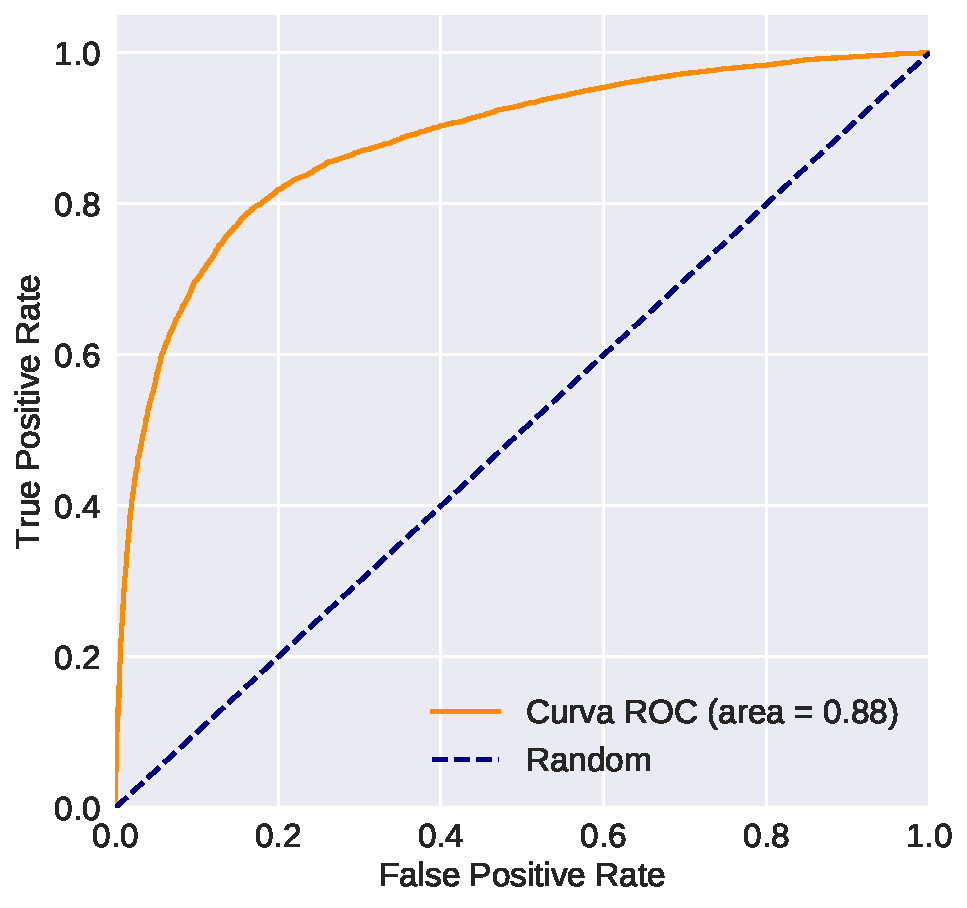
\includegraphics[width=\textwidth]{documents/latex/figures/3/integral/auc_integral.pdf}
    \caption{Curva AUC del algoritmo Random Forest del Dataset Integral. La línea punteada corresponde a un predictor Random.}
    \label{fig:auc_integral}
\end{subfigure}
\hfill
\hfill
\begin{subfigure}[b]{0.9\textwidth}
    \centering
    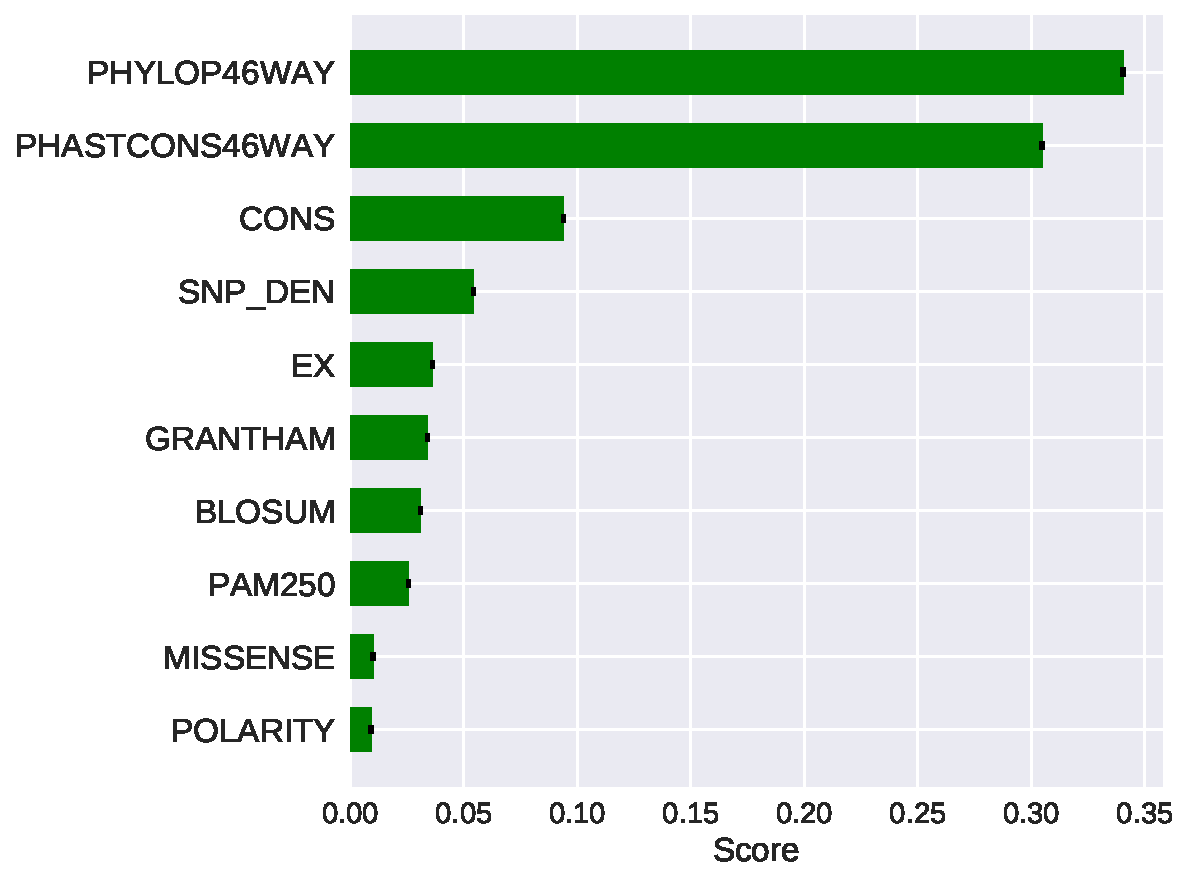
\includegraphics[width=\textwidth]{documents/latex/figures/3/integral/importances_integral.pdf}
    \caption{Los 10 atributos más importantes del Dataset Integral.}
    \label{fig:importances_integral}
\end{subfigure}
\end{figure}





\section{Uniendo las variables al Dataset VarQ}

Una vez generado el Dataset Integral, nos resta evaluar si el modelo mejora aún más sumando las variables de VarQ al conjunto de variables con los que trabajamos.

\pagebreak

\begin{figure}[H]
\centering
\begin{subfigure}[b]{0.8\textwidth}
    \centering
    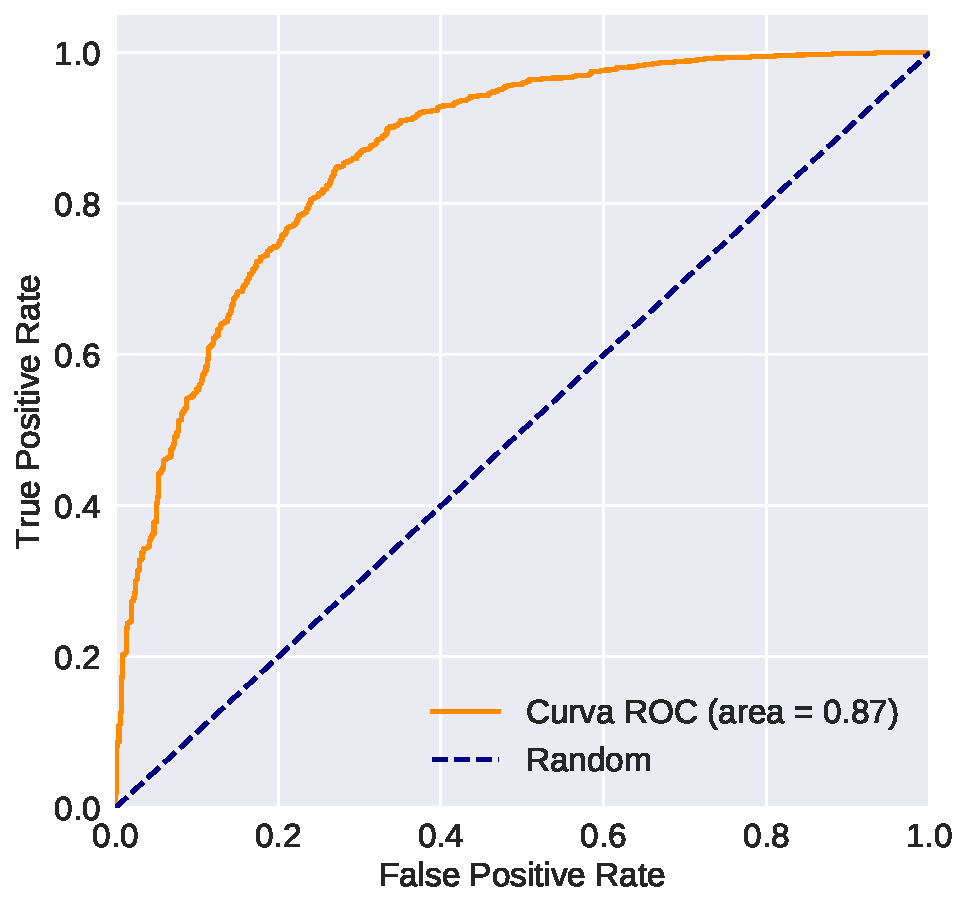
\includegraphics[width=\textwidth]{documents/latex/figures/3/integral_varq/auc_varq_integral.pdf}
    \caption{Curva AUC del algoritmo Random Forest del Dataset Integral. La línea punteada corresponde a un predictor Random.}
    \label{fig:auc_integral_varq}
\end{subfigure}
\hfill
\hfill
\begin{subfigure}[b]{0.9\textwidth}
    \centering
    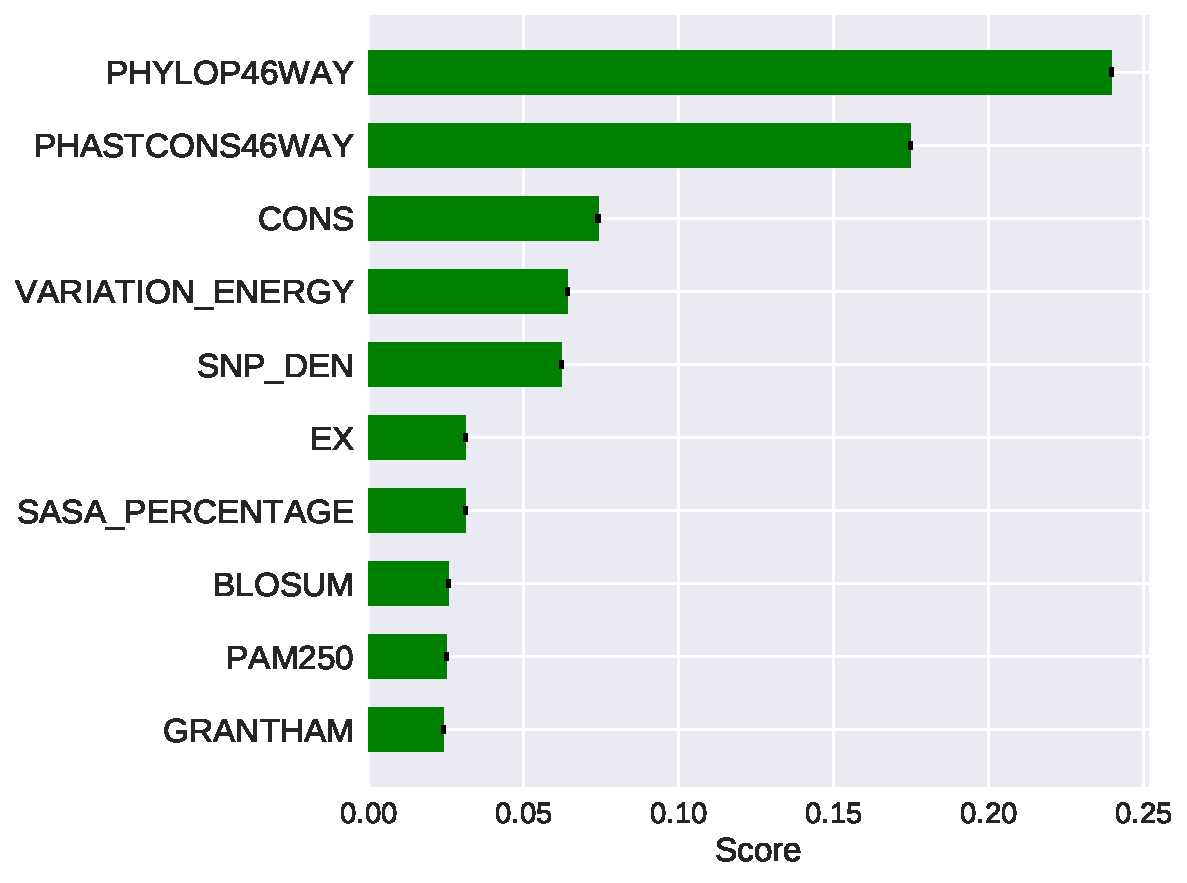
\includegraphics[width=\textwidth]{documents/latex/figures/3/integral_varq/importances_varq_integral.pdf}
    \caption{Los 10 atributos más importantes del Dataset Integral.}
    \label{fig:importances_integral_varq}
\end{subfigure}
\end{figure}






